% ---------------------------------------
%
%    Beispieldiplomarbeit
%
%    - text kann gel{\"o}scht, und mit eigenen Inhalten gef{\"u}llt werden. 
%	In dieser Datei kann die gesamte Konfiguration durchgeführt werden.*
%	
%
%    *mit Ausnahme der spezifischen Optionen in natbib.cfg, die nicht von Interesse sein sollten
% ---------------------------------------

\documentclass[
    smallheadings,  % kleinere {\"U}berschriften
    twoside,        % einseitig, nur rechte seiten
    liststotoc,     % listen in inhaltsverzeichnis aufnehmen
    bibtotoc,       % literaturverzeichnis in inhltsvz. aufnehmen
    headsepline,     % trennlinie unter kopfzeile
    12pt	%Schriftgröße
    ]{scrbook}

\usepackage{a4}  %a4 Seitenformat benutzen
\usepackage[left=4cm,right=2.5cm,top=3.7cm,bottom=4cm]{geometry}
\usepackage[english, ngerman]{babel} %Verwende deutsche und amerikanische Silbentrennung
\usepackage[utf8]{inputenc} %damit k{\"o}nnen Umlaute ganz normal geschrieben werden. 
\usepackage[numbers,square]{natbib}
\usepackage{amssymb}
\usepackage{textcomp}

\usepackage{csquotes}
\usepackage{listings} %Fuer Codelistings
\usepackage{subfigure} %f{\"u}r mehrteilige Grafiken
\usepackage{epsfig}    %damit funktioniert das einbinden von grafiken {\"u}ber epsfig.
\usepackage{graphicx}     % zum einbinden von grafiken
\graphicspath{{grafiken}{../}{kapitel}} %da sind m{\"o}gliche bilder fuer den includegraphics-Befehl zu finden (man muss dann nicht den ganzen Pfad bei includegraphics angeben. 

\usepackage{multirow}     %fuer kompliziertere Tabellen
\usepackage{longtable}	%fuer kompliziertere Tabellen
\usepackage{rotating}	%enable landscape pages
\usepackage{framed}
\usepackage{scrpage2}     % paket f{\"u}r kopf- und fu{\ss}zeilen
\pagestyle{scrheadings}   % kopzeilenseitenstil

%\usepackage{ifpdf} %provides the switch ``ifpdf'' to determine if latex or pdflatex is executed
%see ftp://ftp.ctan.org/tex-archive/macros/latex/contrib/oberdiek/ifpdf.pdf or doc folder

\usepackage{float} % adds location parameter [H] to [htb] to force figures and tables to a location, no floating

%%%% use hyperlinks and adjust settings, see http://en.wikibooks.org/wiki/LaTeX/Hyperlinks and
% ftp://tug.ctan.org/tex-archive/macros/latex/contrib/hyperref/doc/manual.pdf
\usepackage[
a4paper=true, % a4
pdftitle={Leveraging Continuous Integration process to improve Software Reuse}, %title to display for pdfs
pdfauthor={Piero A. Divasto Martínez}, %set author
%dvipdfmx, % must be used if pdf is created from the dvi file rather than by running pdflatex. Otherwise links won't work
colorlinks,% set link color for all links to black, i.e. invisible but working links
citecolor=black,%
filecolor=black,%
linkcolor=black,%
urlcolor=black, %
plainpages=false, %used with pdfpagelabels to make pdf readers show roman and arabic page numbers correctly
pdfpagelabels, %used with plainpages=false to make pdf readers show roman and arabic page numbers correctly
%pagebackref=true %false: no back-references in bibliography to citations in text
]{hyperref} %include hyperlinks for citations, urls, and references
%CAUTION: breaks color settings in dvi, pdf works fine
%%%%end: use hyperlinks

\usepackage{setspace}
\usepackage{url}          % fuer urls: schreibweise ist z.B. \url{http://www.uni-mannheim.de}
%\urlstyle{same} % makes urls in the same font as the rest of the text
\usepackage{xcolor}
\usepackage{minted}

\usepackage{titlesec}

%Automatisch Abkürzungsliste generieren: 2x latex, makeindex myfile.nlo -s nomencl.ist -o myfile.nls, 2x latex
\usepackage{nomencl} % um Abkürzungen aufzunehmen: \abbrev{PDA}{personal digital assistant}
\let\abbrev\nomenclature
\renewcommand{\nomname}{List of Abbreviations} %Titel der Liste hier ändern, eine von zwei Optionen nutzen
%\renewcommand{\nomname}{Abkürzungsverzeichnis} %Titel der Liste hier ändern, eine von zwei Optionen nutzen
\setlength{\nomlabelwidth}{.25\hsize}
\renewcommand{\nomlabel}[1]{#1 \dotfill}
\setlength{\nomitemsep}{-\parsep}
\makenomenclature
\newcommand{\Listofabbrev}{
\printnomenclature
\newpage
}

\usepackage{enumitem}


%Inhaltsverzeichnis
\usepackage
%[
%tocfullflat,			%alle Eintraege left-aligned, alternativ: tocflat
%tocbreakscareless		%page break between toc entry allowed
%]
{tocstyle}			%mehr Kontrolle ueber Inhaltsverzeichnis
\usetocstyle{allwithdot}	%ensure there are dots in table of contents, alternativ: noonewithdot, nopagecolumn
% docu http://www.tug.org/texlive/devsrc/Master/texmf-dist/source/latex/koma-script/tocstyle.dtx
\setcounter{secnumdepth}{3} %numbering up to fifth level in table of contents
\setcounter{tocdepth}{3} %show entries in toc up to fifth level (subsubsubsubsection)


\setlength{\parindent}{0pt}		% Einzug fuer neuen Absatz
\setlength{\parskip}\medskipamount % Abstand neuer Absatz, besser als explizite Angabe in pt

\onehalfspacing %Zeilenabstand 1,5


% kapitel{\"u}berschriften in schriftart mit serifen
\setkomafont{sectioning}{\normalfont\normalcolor\bfseries}

% gestaltung der kopfzeilen
\ohead{\pagemark}
\ifoot{}
\cfoot{}
\ofoot{} 
\cohead{}
\ihead{\headmark}
\setkomafont{pagehead}{\normalfont\bfseries}
\setkomafont{pagenumber}{\normalfont\bfseries}
\automark{section}

% ----- ende der pr{\"a}ambel ----------------------------------






\begin{document}  % dokument f{\"a}ngt an
\selectlanguage{english} %englische Silbentrennung, fuer deutsche Arbeiten: \selectlanguage{ngerman}
\frontmatter      % vorspann, kapitel r{\"o}misch nummeriert
\newgeometry{margin=3cm}
% Die Titelseite der Arbeit

\begin{titlepage}

\begin{center} % zentrieren

  % Logo der Universit{\"a}t Mannheim
  \begin{figure}[ht]
    \centering
    
\includegraphics[width=.6\textwidth]{grafiken/unilogo}
  \end{figure}
  
  % Vertikaler Zwischenraum
  \bigskip
  \vfill 
  \begin{framed}
  % Titel der Arbeit und Typ der Arbeit, umrandet
    \begin{center}
     \textsc{{\Large This thesis's title \\ Subtitle\\}}
                                % Letztes \\ ist wichtig, beginnt eine neue Zeile f{\"u}r die Art der Arbeit
  
      \bigskip
  
                                % Art der Arbeit, ggf. auszutauschen gegen Seminar- oder Doktorarbeit
      \textbf{Term Paper}
    \end{center}
    \end{framed}
    \vfill
    \vfill
  
  % Daten des Erstellers, Einreichungsdatum
  % in einer Tabelle ausgerichtet
  \begin{tabular*}{0.62\textwidth}{r@{\extracolsep{\fill}}l}
   submitted: &\ January 2004\\\\
    by: &\ Martin Mustermann\\
    &\ born March 28th 1984\\
    &\ in Eberbach\\
    \\
    Student ID Number: &\ 012345\\
  \end{tabular*}
  \vfill
  \vfill
  
  % Unten: Kontaktdaten des Lehrstuhls f{\"u}r Wirtschaftsinformatik 1
  
  \rule{\textwidth}{.4pt}\\ % vertikale Linie
  University of Mannheim\\
  Chair of Business Administration and Information Systems\\
  D -- 68131 Mannheim\\
  Phone: +49 621-181-1691, Fax +49 621-181-1692\\
  Internet: \url{http://heinzl.bwl.uni-mannheim.de}
\end{center}

\end{titlepage} % Ende des Titelblatts

%%% Local Variables: 
%%% mode: latex
%%% TeX-master: "~/Documents/DA-Vorlage/beispiel/da-beispiel"
%%% End: 
     % titelseite einbinden
\restoregeometry
\chapter{Abstract}
On the one hand we have the Douglas McIlroy's vision \cite{McIlroy1968} of a software system composed of already existent components. Where you basically put different components, that already exist, together in order to form the system is being built. Although the IT industry has tried for many years to improve the speed and reduce cots of software development by reusing components, this vision is still the exception rather than the rule. On the other hand we have Continuous Integration which is a software development practice where members of a team integrate their work frequently, usually each person integrates at least daily, thus leading to multiple integrations per day. Each integration is verified by an automates build (including test) to detect integration errors as quickly as possible. In this work we present a novel approach that improve the reuse of software by leveraging continuous integration process. Also we present an unobtrusive tool as a proof-of-concept that extracts interface signatures and test classes from a given project, which are sent to a code-search engine to retrieve similar components based on text-driven and test-driven search techniques  % abstract einbinden
\tableofcontents            % inhaltsverzeichnis
\listoffigures              % abbildungsverzeichnis
\listoftables               % tabellenverzeichnis

%\clearpage %tell toc that there is a pagebreak after list of tables, however the hyperlink still points to the wrong page

\addcontentsline{toc}{chapter}{\nomname} %abkuerzungen ins inhaltsverzeichnis

% Abbreviations
\nomenclature{$CI$}{Continuous Integration}
\nomenclature{$CD$}{Continuous Delivery}
\nomenclature{$VCS$}{Version Control System}
\nomenclature{$TDD$}{Test-driven Development}
\nomenclature{$TFD$}{Test-first Development}
\nomenclature{$VCP$}{Version Control Platform}
\nomenclature{$CVS$}{Concurrent Versions System}
\nomenclature{$SCM$}{Source Control Management}
\nomenclature{$CC$}{Creative Commons}

\Listofabbrev % liste der abkuerzungen erstellen

\mainmatter       % hauptteil, kapitel lateinisch nummeriert
%\include{kapitel/content}
\selectlanguage{english} % jetzt sprechen wir wieder englisch
\chapter{How to use the template}
\label{chap:howto}

This is an evolved latex template. Chapters 2 and 3 remain from former versions of this template. In this first chapter a very short overview on basic handling of this template is given. All users of kile are lucky as configuration instructions are provided only for this latex editor.
\section{General structure}
\label{sec:generalStructure}
The structure provided with this template and recommended for use is as follows: The main TeX file ``arbeit.tex" is placed in the root directory of the project. All configuration tasks should be done in this main file. This way, one may concentrate on writing rather than bothering with formatting the layout in the single chapters. Figures are placed in the folder ''grafiken`` and the chapters as single files in ''kapitel``. In the directory ''literatur`` there are bibliography styles and the bib file ''lit.bib`` that contains your references. More detailed information on some packages used by the template can be found in directory ''doc``. 

\section{Compilation}
\label{sec:compilation}
This template should be used with latex/pdflatex (text, figures), bibtex (bibliography) and makeindex (table of contents). It is recommendable to use a compilation sequence for the root file as follows: latex (2x), bibtex, makeindex, latex(2x). If you want to create a pdf file just run pdflatex after a full compilation sequence. However, this requires that the figures you use are present in two formats, one that can be handled by latex and one for latex. For example, you can use the eps and the pdf formats.

Furthermore, you must configure your invocation of makeindex. It should look like: ''makeindex arbeit.nlo -s nomencl.ist -o arbeit.nls''. For kile you may configure the options of makeindex in Settings -- Configure Kile -- Tools -- Build -- MakeIndex to ''\%S.nlo -s nomencl.ist -o \%S.nls``. The files arbeit.nlo and arbeit.nls must be present but may be empty. So if there are no files with the main file's name and the extensions nlo and nls just create empty ones.

It is convenient to work with dvi files as working copies and to run pdf latex only once in a while to see a pdf file with hyperlinks. DVIs are ugly and have more bugs but they are faster to compile and to render. Moreover, the longer you have stared on an ugly dvi file, the happier you are when the pdf appears and looks nice.

 To define a compilation sequence in kile go to Settings -- Configure Kile -- Tools -- Build -- QuickBuild. There you may set the sequence, e.g.\ to: latex, latex, bibtex, makeindex, latex, latex, xdvi (where xdvi is a dvi viewing program). 
 
 In short, there are two possible compilation sequences.
 
 Compilation sequence for dvi:
 \begin{enumerate}
  \item latex (2x)
  \item bibtex
  \item makeindex (make sure it is configured correctly or you will catch odd errors)
  \item latex (2x)
 \end{enumerate}
 
 Compilation sequence for pdf:
 \begin{enumerate}
  \item latex (2x)
  \item bibtex
  \item makeindex (make sure it is configured correctly or you will catch odd errors)
  \item latex (2x)
  \item pdflatex
 \end{enumerate}
  


\section{Languages}
\label{sec:languages}
This template is configurable for English and German papers. The entire configuration should be done in the root file ''arbeit.tex``. To set a language, there are three commands to edit in the root file: \begin{enumerate}
                                                                                                             \item the bibliography style at the end of the document must fit the language. For each language there is at least one predefined version you may choose. Look for the ''bibliographystyle`` tag. Comments are in place explaining what they are about.
\item change the headline of the list of abbreviations to a suitable version. Look for the ''nomname`` tag.
\item use an appropriate selectlanguage command and remove the other ones.
                                                                                                             \end{enumerate}


\section{Abbreviations}
\label{sec:abbreviations}

The package nomencl is used to create a list of abbreviations. To add an entry to the list use ``abbrev``. This is an example for ''telecommunications company''\abbrev{TC}{telecommunications company}. To create the list run the compilation sequences as defined above.


\section{Citations}
\label{sec:citations}

The citation style used is called natbib and can be used to create numerical and author-year citations. To create the bibliography the bibliography style natdin is used as a basis for German papers, apalike2 for English ones. The respective .sty-file for natdin is located in the directory literatur. More information can be found on \url{http://merkel.zoneo.net/Latex/natbib.php} or in the directory ``doc''. Adjust the bib styple in the file arbeit.tex to fit your needs. Read the comments, some may help you. 

\subsection{The bib file}
\label{subsec:theBibFile}

The bibliography file is placed in the directory literatur and is called lit.bib. In the lit.bib file you will find different annotations to be used for different kinds of papers. This effects their representation in the bibliography. Some comments can be found in this file, too.

\subsection{Citations}
\label{subsec:citations}

Talking about a paper one may want to do a citation in the text using citet as in \citet{COMITY}. Alternatively parenthesis may be useful \citep{tannenbaum}. It is also possible to add more information like the pages of a book one refers to \citep[pp. 222-333]{tannenbaum}. \citet{ECORA}, \citet{random}, \citet{habil} and \citet{master} are in text citations. There is the Web Ontology Language \abbrev{OWL}{Web Ontology Language} \citep{OWL} as an example of an electronic resource.

There are three slightly different bib styles in the directory literatur. First, the native natdin.bst for DIN citations in German. Second, a slightly modified version ''natdinCustomized''. This style has minor changes in punctuation and is therefore not conform to DIN 1505. Third, an English translation of the latter is provided. Choose your bibliographystyle at the end of the root file (arbeit.tex). For English papers, apalike2 looks quite nice.

Several options for citations and the bibliography may be configured in the root file as usepackage parameters for natbib, e.g.\ the type of brackets used. See natnotes.pdf in the directory ``doc'' for more information. Additionally, for very detailed configuration it is possible to use the file ``natbib.cfg'' in the root directory to override predefined parameters.

\section{Table of Contents}
\label{sec:toc}

To create a nice table of contents the package tocstyle is used. Configuration options can be found in tocstyle.pdf located in ``doc''.

\section{Troubleshooting}
\label{sec:troubleshooting}

Use the provided information in log messages. If changes you made do not appear in the document, recompile twice (including 2x latex, bibtex, makeindex). Additionally, you may delete all automatically created files, especially the .aux, .bbl, .out, .toc, .lof, .lot, and .ilg files. Make sure you do not delete .tex, .nlo, .nls, .sty, and .cfg files. Moreover, ensure you have used the right compilation sequence and configured makeindex correctly. If you are using dvi, have a look at a pdf if the problem is also present there, often they are not. 
\chapter{Software Reuse}
\label{chap:sw-reuse}

Software reuse is a concept that

\section{Citations}
\label{sec:citations}

The citation style used is called natbib and can be used to create numerical and author-year citations. To create the bibliography the bibliography style natdin is used as a basis for German papers, apalike2 for English ones. The respective .sty-file for natdin is located in the directory literatur. More information can be found on \url{http://merkel.zoneo.net/Latex/natbib.php} or in the directory ``doc''. Adjust the bib styple in the file arbeit.tex to fit your needs. Read the comments, some may help you. 

\subsection{The bib file}
\label{subsec:theBibFile}

The bibliography file is placed in the directory literatur and is called lit.bib. In the lit.bib file you will find different annotations to be used for different kinds of papers. This effects their representation in the bibliography. Some comments can be found in this file, too.

\subsection{Citations}
\label{subsec:citations}

Talking about a paper one may want to do a citation in the text using citet as in \citet{COMITY}. Alternatively parenthesis may be useful \citep{tannenbaum}. It is also possible to add more information like the pages of a book one refers to \citep[pp. 222-333]{tannenbaum}. \citet{ECORA}, \citet{random}, \citet{habil} and \citet{master} are in text citations. There is the Web Ontology Language \abbrev{OWL}{Web Ontology Language} \citep{OWL} as an example of an electronic resource.

There are three slightly different bib styles in the directory literatur. First, the native natdin.bst for DIN citations in German. Second, a slightly modified version ''natdinCustomized''. This style has minor changes in punctuation and is therefore not conform to DIN 1505. Third, an English translation of the latter is provided. Choose your bibliographystyle at the end of the root file (arbeit.tex). For English papers, apalike2 looks quite nice.

Several options for citations and the bibliography may be configured in the root file as usepackage parameters for natbib, e.g.\ the type of brackets used. See natnotes.pdf in the directory ``doc'' for more information. Additionally, for very detailed configuration it is possible to use the file ``natbib.cfg'' in the root directory to override predefined parameters.
\chapter{Continuous Integration}
\label{chap:ci}

In this chapter we will explain what Continuous Integration (CI) means, we will describe the process steps, its benefits and challenges. Finally we will explain how CI can be leveraged in order to improve Software Reuse.

\section{What is Continuous Integration?}
\label{sec:ci-def}

The term can be found in the context of micro-processes development in the work of \cite{Booch2007}. Then it was adopted by Kent Beck in his definition of Extreme Programming \citep{Beck1999}. However, it was Martin Fowler who was credited with establishing the current definitions of the practices. Fowler defines CI as following:

CI is a software development practice where members of a team integrate their work frequently, usually each person integrates at least daily, thus leading to multiple integrations per day. Each integration is verified by an automates build (including test) to detect integration errors as quickly as possible. Many teams has found that this approach leads to significantly reduced integration problems and allows a team to develop cohesive software more rapid\citep{Fowler2006}.

Continuous Integration emerges as a solution for the painful moment of software integration. Although the process of integrating software is not a problem for a one-person project, when it increases in complexity it becomes more problematic. For example, in the old days, a software was divided in modules and each of them were developed independently, once they done, those modules were put together in one step at the end of the project. Doing that led to all sorts of software quality problems, which are costly and often lead to project delays \citep{Duvall2007}.

This step of module integration was a tense moment as errors and failures appeared and they were difficult to find and fix at that stage of the development. In this manner, instead of waiting till the end of modules development to integrate, CI proposes to integrate frequently, usually one person should integrate at least once a day.

Therefore we can break up the CI workflow in the following steps \citep{Fowler2006}:

\textbf{CI Workflow:}

\begin{itemize}
\item Developers check out code into their private workspaces
\item When done, commit the changes to the repository
\item The CI server monitors the repository and checks out changes when they occur.
\item The CI server builds the system and runs unit and integration tests.
\item The CI server releases deployable artifacts for testing.
\item The CI server assigns a build label to the version of the code it just built.
\item The CI server informs the team of the outcome of the build.
\item In case the build or test failed, the team fixes the issue at the earliest opportunity.
\item Continue to continually integrate and test throughout the project.
\end{itemize}

This uncomplicated workflow helps the development team to focus on the current code change till it is verified and validated. Moreover, it provides continuous feedback on the quality of the code.

\subsection{CI Tools}

Although the CI is tool agnostic, the selection of them depends on the project, framework in use, skill-set of the stakeholders and other factors. There are however two must-have tools of any CI system: (1) the version control system (VCS) and (2) the CI server.

The most popular VCS are Git, Mercurial and SVN. On top of them, we can find Version Control Platforms (VCP) such as Github, Gitlab or Bitbucket. In terms of CI servers, we can find Jenkins, Hudson, GoCD as open source projects; TravisCI, CircleCI, CodeShip and Team City as commercial tools.

Therefore choosing the appropriate tools is about finding the balance between price, setup, configuration efforts, ease-of-use, integration capabilities between the selected tools, framework suitability and maintainability in respect to current code base.

\subsubsection{Git}
Within the several different VCSs available, Git is one of the most popular\footnote{https://rhodecode.com/insights/version-control-systems-2016 (accessed: 14.01.2017)}. Git emerges in 2005 as an alternative to BitKeeper\footnote{https://www.bitkeeper.com/ (accessed: 13.01.2017)} after the break of the relationship between the commercial company behind BitKeeper and  the community that developed the Linux kernel \citep{Chacon2009}.

The main difference between Git and the other VCSs is the way it thinks about its data. Other VCSs such as Subversion, CVS, Perforce, and so on, think of the information they keep as a set of files and the changes made to each file over time. On the other hand, Git thinks its data like a set of snapshots of a miniature file system. Therefore, every time a user commits, or save the state of the project, Git basically takes a picture of what all the files look like at that moment and store a reference to that snapshot. In addition, Git has three main states where the files can reside in: committed, modified, and staged. Committed means that the data is stored in the local database. Modified means that the file was modified but it has not been committed yet. And staged means that the modified file has been marked to go into the next commit \citep{Chacon2009}. The figure \ref{fig:git-sates} depicts these three states.

\begin{figure}[ht]
	\centering
    \includegraphics[width=\textwidth]{grafiken/git-states}
    \caption{The three main states of Git \citep{Chacon2009}}
    \label{fig:git-sates}
\end{figure}

The git directory is the core of Git as it is where the metadata and object database for a project is stored. The working directory is a single checkout of one version of the project. Finally, the staging area is a file which is generally stored in the Git directory. This file contains information about what will go into the next commit.

\subsubsection{Github}

Github\footnote{https://github.com/ (accessed: 13.01.2017)} is a web-based Git repository hosting service, which offers all the functionality of Git and its own features. It provides several collaboration tools such as wikis, bug tracking, feature requests, and task management as well as access control. Its development started in 2007 as a side project of P. J. Hyett and Chris Wanstrath \citep{Weis2014} and it was officially lunch on the 10th of April in 2008. Since then, Github has gain popularity through the community reaching more than 50 million projects hosted nowadays.

\subsubsection{Jenkins}
Jenkins is an open source automation server developed in Java. It was originally founded in 2006 as \textit{Hudson}, however a disputed with Oracle the community behind Hudson decided to change the project name to Jenkins\footnote{http://archive.is/fl45 (accessed: 13.01.2017)}.

Jenkins enables developers to reliable build, test, and deploy their software. Its extensible and plugin-based architecture has permitted to create a tons of plugins to adapt the CI server to a multitude of build, test, and deployment automation workloads. In 2015, Jenkins surpassed 100.000 known installation making it the most widely deployed automation server\footnote{https://jenkins.io/press/ (accessed: 13.01.2017)}. 

\section{Benefits in adopting CI/CD}
\label{ci-benefits}

Several are the benefits that come with the adoption of Continuous Integration in a software project. In this section we will describe five areas that are improved after CI implementation \citep{Rejstrom2016}. It is important to point out that these benefits come along with other practices such as agile transformation \citep{Laanti2011} and lean software development \citep{Poppendieck2003}.

\begin{itemize}
\item Shorter time-to-market: Many benefits come with the adoption of frequent releases. With fast and frequent releases is possible to get feedback quickly from customer and market, thus the organization gets better understanding of their needs expectations \citep{Neely2013}. With that is possible to focus on the most relevant features. Another benefit of delivering frequently is waste reduction as features can be deployed as soon as they are done \citep{Leppanen2015}. Furthermore, with frequent releases is possible to experiment with new features easily and with low impact \citep{Neely2013}.
\item Rapid feedback: With frequent releases is possible to show progress to customers and by that get feedback quickly. With that the development team can focus on important features instead of waste time in features that are not relevant for the customers or the market.
\item Improved software quality: Researches have reported a decreased in the number of open bugs and production incidents after adopting CI practices \citep{Mantyla2015} and the link between software quality improvement and the heavy reliance on automated test combined with smaller more manageable releases \citep{Leppanen2015}.
\item Improved release reliability: In the work of \cite{Neely2013} was proved that a working deployment pipeline along with intensive automated testing and fast rollback mechanism possitively affects release reliability and quality. With small and frequent releases fewer things can go wrong in a release according to \cite{Fowler2013}. In fact, reduction in the stress of developers and other stakeholder have been found by adopting CI \citep{Neely2013} \citep{Chen2015}.
\item Improved developer productivity: By automating deployment process, environment configuration and other non-value adding tasks, significant time saving for developers have been observed \citep{Rodriguez2016}. Also, in the work of \cite{Humble2010} was observed that although the setup cost of a deployment pipeline can be high, after it is setup developers can focus on value adding software development works.
\end{itemize}

\section{Challenges in adopting CI/CD}
\label{ci-challenges}

Adopting CI can be very beneficial for a software project as described above, however we can face some challenges that can jeopardize the successful implementation of it. According to the literature, there are seven common challenges in the implementation of a CI:

\begin{itemize}
\item Change resistance: Transforming the development of a project towards continuous integration practices requires investment and involvement from the entire organization \citep{Rodriguez2016}. Therefore any transformation in how an organization works, will receive a resistance on both a personal level and decision level within the organization.
\item External constraint: As a software project is part of a context, external constraint may appear. Normally customer preferences and domain imposed restrictions are sources of constraints. For example in highly restricted domains, legal regulations may require extensive testing before new version can be allowed to enter production \citep{Rodriguez2016}.
\item QA effort: The automated tests suit needs to be exhaustive enough in order to ensure the quality of what is being built. Thus it can lead to increase QA efforts due to difficulties in managing the test automation infrastructure \citep{Rodriguez2016}.
\item Legacy code: Normally legacy software has not been design for being automatically tested and may cause integration failures which may inhibit the continuous deployment process. The ownership of legacy code might belong to another company or team which shift the testing responsibility and this might delay the deployment process.
\item Complex software: If the complex if the software project is high, then setting up the CI workflow is more challenging \citep{Leppanen2015}.
\item Environment management: Keeping all the environments used in development, testing and production sync and similar can be challenging. This is due to the fact that differences in the environment configuration can lead to undetected issues appear in production. Therefore is essential to have a good configuration management that provisions environments automatically \citep{Leppanen2015}.
\item Manual testing: Although automated tests are very beneficial, some aspects of software need to be manually tested such as security issues, performance and UX/UI. Therefore 	heavy manual testing can impact the overall speed and smoothness of the process \citep{Leppanen2015}.
\end{itemize}

\section{Successful CI practices}
\label{ci-successful-pract}

In order to reduce the risks in adopting CI practices, eight principles, based on several literature reviews, were defined in \citep{Rejstrom2016} which should guide the CI implementation within organizations. These principles are generic solutions which can be adapted in most cases.

\begin{itemize}
\item Automate the build: The task that triggers the whole pipeline is the commit. After each commit, the next step should be build the binaries. The executable that result of the build, should go through the pipeline until it gets validated, verified and deployment ready.
\item Make your build self-testing: 
\item Every commit should build on an integration machine
\item Keep the build fast
\item Keep the build green
\item Test in a clone of the production environment
\item Everyone can see what is happening
\item Automate deployment
\end{itemize}

These 8 principles should guide the CI/CD implementation within organizations. The principles have been stablished as best practices through the validation of these concepts through several literature reviews [\cite{Rodriguez2016}; \cite{Mantyla2015}; \cite{Stahl2014}]. They can be viewed almost as a design pattern for adopting CI/CD, offering a generic solution adaptable to most cases.
\section{Test-Driven Development}
In this section we will explain Test-driven development (TDD). TDD combines test-first development where you write a test before you write just enough production code to fulfill that test, and refactoring. The primary goal of TDD is to think through your requirements or design before your write your functional code (implying that TDD is both an important agile requirements and agile design technique). In the reminder of this section we will explain further the definition of TDD, compare it versus normal testing, and explain why to use TDD.

\subsection{Definition}
The steps of test-first development (TFD) are displayed in the activity diagram of Figure \ref{fig:tfd}. The first step is to quickly add a test. Then it is executed, often the complete test suite although one may decide to run only a subset for the sake of speed, to ensure that the new test fails. After that the developer updates the functional code to make it pass the tests. The fourth step is to run your tests again. If they fail he/she needs to update the functional code and retest. Once the tests pass, the next step is to start over. One may first need to refactor the code if needed, in that case we are turning TFD into TDD.

\begin{figure}[H]
	\centering
    \includegraphics[width=0.5\textwidth]{grafiken/tfd}
    \caption{Test-First Development}
    \label{fig:tfd}
\end{figure}

TDD completely inverts traditional development. When a developer first goes to implement a new feature, the first question that he/she asks is whether the existing design is the best design possible that enables him/her to implement that functionality. If so, he/she proceeds via a TFD approach. If not, he/she refactors it locally to change the portion of the design affected by the new feature, enabling him/her to add that feature as easy as possible. As a result he/she will always be improving the quality of the design, thereby making it easier to work with in the future. Figure \ref{fig:tdd} describes the TDD lifecycle just described.

\begin{figure}[H]
	\centering
    \includegraphics[width=\textwidth]{grafiken/tdd}
    \caption[Test-driven Development lifecycle]{Test-driven Development lifecycle\protect\footnotemark}
    \label{fig:tdd}
\end{figure}

\footnotetext{Test-driven Development lifecycle - \url{http://upload.wikimedia.org/wikipedia/commons/0/0b/TDD_Global_Lifecycle.png} (accessed: 20.02.2017)}

Instead of writing functional code first and then writing testing code, if it is written at all, a developer instead writes test code before the functional code. Moreover, he/she does so in very small steps (i.e. one test and a small bit of proportional functional code at a time). A programmer taking a TDD approach refuses to write a new function until there is a test first that fails because that function is not present yet. In fact, they refuse to add even a single line of code until a test exists for it. Once the test is in place then they do the work required to ensure that the test suite now passes (i.e. new code may break several existing tests as well as the new one). Although it sounds simple, one needs a great discipline because it easy to forget it and write functional code without first writing a new test.

There are two levels of TDD:

Acceptance TDD (ATDD).  With ATDD you write a single acceptance test, or behavioral specification depending on your preferred terminology, and then just enough production functionality/code to fulfill that test. The goal of ATDD is to specify detailed, executable requirements for your solution on a just in time (JIT) basis. ATDD is also called 

Behavior Driven Development (BDD).
Developer TDD. With developer TDD you write a single developer test, sometimes inaccurately referred to as a unit test, and then just enough production code to fulfill that test. The goal of developer TDD is to specify a detailed, executable design for your solution on a JIT basis. Developer TDD is often simply called TDD.

Figure 2 depicts a UML activity diagram showing how ATDD and developer TDD fit together.  Ideally, you'll write a single acceptance test, then to implement the production code required to fulfill that test you'll take a developer TDD approach. This in turn requires you to iterate several times through the write a test, write production code, get it working cycle at the developer TDD level.
\subsection{TDD vs Traditional Testing}
TDD is primarily a specification technique with a side effect of ensuring that your source code is thoroughly tested at a confirmatory level.  However, there is more to testing than this.  Particularly at scale you'll still need to consider other agile testing techniques such as pre-production integration testing and investigative testing. Much of this testing can also be done early in your project if you choose to do so (and you should). 
With traditional testing a successful test finds one or more defects. It is the same with TDD; when a test fails you have made progress because you now know that you need to resolve the problem. More importantly, you have a clear measure of success when the test no longer fails. TDD increases your confidence that your system actually meets the requirements defined for it, that your system actually works and therefore you can proceed with confidence. 
As with traditional testing, the greater the risk profile of the system the more thorough your tests need to be. With both traditional testing and TDD you aren't striving for perfection, instead you are testing to the importance of the system. To paraphrase Agile Modeling (AM), you should "test with a purpose" and know why you are testing something and to what level it needs to be tested.  An interesting side effect of TDD is that you achieve 100\% coverage test – every single line of code is tested – something that traditional testing doesn’t guarantee (although it does recommend it).  In general I think it’s fairly safe to say that although TDD is a specification technique, a valuable side effect is that it results in significantly better code testing than do traditional techniques.   
\subsection{Why TDD?}
A significant advantage of TDD is that it enables you to take small steps when writing software. This is a practice that I have promoted for years because it is far more productive than attempting to code in large steps. For example, assume you add some new functional code, compile, and test it.  Chances are pretty good that your tests will be broken by defects that exist in the new code. It is much easier to find, and then fix, those defects if you've written two new lines of code than two thousand. The implication is that the faster your compiler and regression test suite, the more attractive it is to proceed in smaller and smaller steps. I generally prefer to add a few new lines of functional code, typically less than ten, before I recompile and rerun my tests.
I think Bob Martin says it well “The act of writing a unit test is more an act of design than of verification.  It is also more an act of documentation than of verification.  The act of writing a unit test closes a remarkable number of feedback loops, the least of which is the one pertaining to verification of function”.
The first reaction that many people have to agile techniques is that they're ok for small projects, perhaps involving a handful of people for several months, but that they wouldn't work for "real" projects that are much larger.  That’s simply not true. Beck (2003) reports working on a Smalltalk system taking a completely test-driven approach which took 4 years and 40 person years of effort, resulting in 250,000 lines of functional code and 250,000 lines of test code.  There are 4000 tests running in under 20 minutes, with the full suite being run several times a day. Although there are larger systems out there, I've personally worked on systems where several hundred person years of effort were involved, it is clear that TDD works for good-sized systems.
\subsection{Tools}
The following is a representative list of TDD tools available to you.  Please email me with suggestions. I also maintain a list of agile database development tools.

cpputest
csUnit (.Net)
CUnit
DUnit (Delphi)
DBFit
DBUnit
DocTest (Python)
Googletest
HTMLUnit
HTTPUnit
JMock
JUnit
Moq
NDbUnit
NUnit
OUnit
PHPUnit
PyUnit (Python)
SimpleTest
TestNG
TestOoB (Python)
Test::Unit (Ruby)
VBUnit
XTUnit
xUnit.net
\section{Microservices}

Microservices is a software architecture is usually linked to Martin Fowler in its article \citep{Fowler2014}. It is an architectural styles that aim to develop applications as a suite of small services independently of each other. Each of this services runs in its process and they communicate with lightweight mechanisms (e.g. HTTP resource API). These services are built around business capabilities and independently deployed by fully automated deployment machinery. Also there is a bare minimum of centralized management of these services, which may be written in different programming languages and use different data storage technologies \citep{Fowler2014}.

This architectural style emerges as a solution to the monolithic style due to its problems. An application built using monolithic architectural style is considered as a single unit with normally three main parts (figure \ref{}): a client-side user interface (i.e. HTML, CSS, JavaScript running on user's machine), a database and a server-side application. The latter is a monolith as it handles HTTP request, execute domain logic, retrieve and update data from the database, and populates and/or select the HTML views sent to the client-side. As it is a single logical executable, any changes made in the system, no matter the size of it, require a build and a deploy of the whole server-side application. It is hard to keep a good modular structure, making it harder to keep changes that must affect one module within that module. Also it is hard to scale as it is necessary to scale the entire application rather than parts of it requiring greater resources. These problems are causing frustrations on people that are using this style, specially nowadays when applications are deployed to the cloud, leading to the microservices architectural style.

\subsection{Characteristics of a Microservice Architecture}
In the work of Fowler and Lewis \citep{Fowler2014} described a list of common characteristic of applications built using microservice architectural style. It is important to point out that all the applications using this style must confirm every characteristic of this list.

\begin{description}[style=nextline]
\item[Componentization via Services] \hfill \
First of all it is important to explain the differences between libraries and services as the primary way of componentizing is by breking down software into services. On the one hand libraries are components that are linked into a application and called using in-memory function calls. On the other hand services are out-of-process components which communicates with a mechanism such as a web service request, or remote procedure call \citep{Fowler2014}.

Splitting a software into services brings benefits such as services as components are independently deployable making it easy for changes, or services have more explicit component interfaces by using explicit remote call mechanisms. 
\item[Organized around Business Capabilities] \hfill \
Normally in monolithic applications the development teams are divided by technology layers such as front-end team, server-side team and database team. However when team are divided in this way, even simple changes can lead to a cross-team project taking time and budgetary approval.

In Microservices approach this is taken in a different way by dividing the application into services organized around business capability. Thus services involve all needed for that business area, including user-interface (UI), database, business logic, and any other external collaboration. Therefore each teams are cross-functional, including the full range of skills required for the development of it.
\item[Products not Projects] \hfill \
Usually software development follows a project model where the objective is to deliver some piece of software which, when it is done, it is delivered to a maintenance team and the development team is disbanded.

Microservices approach follows the product model instead of project model. In the product model the development team takes full responsibility of the software, in other words it owns the product. This results in day-to-day contact of the developers with the users as they have to take on at least some of the support. Moreover this mentality ties in with the linkage to business capabilities as the focus is on how the software can assist its users to enhance the capabilities instead on put the focus on a list of functionality.
\item[Smart endpoints and dumb pipes] \hfill \
Microservices 
\item[Decentralized Governance] \hfill \

\item[Decentralized Data Management] \hfill \

\item[Infrastructure automation] \hfill \

\item[Design for failure] \hfill \

\item[Evolutionary design] \hfill \
\end{description}

\chapter{Usage Scenario}
\label{usage-scenario}
Before getting into the approach presented in this work, we will propose a usage scenario to strength and motivate it. The following scenario is based on the usage scenario found in \cite{Kessel2016}.

First of all we will assume that the test software project has the following characteristics. The project has adopted Continuous Integration as we described in Section \ref{chap:ci}, using Git as Version Control System, Jenkins as CI Server, and Java as programming language. Moreover the software is developed following the Test-driven development process.

Envisage the following scenario in which a development team is working or has code ownership of a web service application, and recognizes that she/he requires the ability to encode and decode information in the common Base64 format (e.g., the Base64 variant used in MIME transfer encoding \cite{rfc2045}).

As the project is being developed using TDD, developers create a test case that defines a function before it is implemented. For instance, if we follow the scenario, a member of the team will implement the method \emph{encode} which accept an array of bytes decoded in Base64 and it will return an array of chars which represents the input decoded. Moreover the method \emph{decode} that receives an array of chars and returns an array of bytes that represents the input encoded will need to be implemented too. However, as they are using TDD, this member must create a test of these methods before writing functional code. Listing \ref{Base64.java} represents the methods \emph{encode} and \emph{decode} and Listing \ref{Base64Test.java} represents the test class for these methods.

\lstinputlisting[
  language=Java, numbers=left, stepnumber=5, firstnumber=1, breaklines=true, 
  basicstyle=\footnotesize,
  numberstyle=\tiny,
  caption={Base64.java},
  captionpos=b,
  label=Base64.java
]
{code/Base64.java.txt}

\lstinputlisting[
  language=Java, numbers=left, stepnumber=5, firstnumber=1, breaklines=true, 
  basicstyle=\footnotesize,
  numberstyle=\tiny,
  caption={Base64Test.java},
  captionpos=b,
  label=Base64Test.java
]
{code/Base64Test.java.txt}

After that, this programmer will write enough code to fulfill the test case. This enough code neither need to be the \emph{best} nor the last version, because the next step will be to refactor it. Listing \ref{Base64.B.java} represents the enough code to pass the test.

\lstinputlisting[
  language=Java, numbers=left, stepnumber=5, firstnumber=1, breaklines=true, 
  basicstyle=\footnotesize,
  numberstyle=\tiny,
  caption={Base64.java with Implementation to Pass the Test Case},
  captionpos=b,
  label=Base64.B.java
]
{code/Base64.java.B.txt}

Additionally, as the team adopted CI, developers should commit often the changes to the Git server. After adding enough functional code to fulfill the test case, the developer is able to push new code to the Git server. This action triggers the CI server which checkouts the code and runs the unit tests available. Therefore going along with the example given above, the class \emph{Base64.java} and the test class \emph{Base64Test.java} should be committed to the repository.

From this simple scenario emerge the following questions:

\begin{description}[style=nextline]
\item[How might the team realize that what they are working on has not been developed already?] \hfill \
If we follow the example, the implementation of encode and decode in Base64 is very easy to find, however that does not mean that the developer is aware of that at the moment he/she is developing. Therefore it would be very useful that an automated tool analyzes the code and recommends similar components that implement the functionality being developed.
\item[How might we seize continuous integration in order to improve chances of reusing software?] \hfill \
Continuous integration process seems to be a very good opportunity for software reuse. According to CI workflow explained in Section \ref{chap:ci}, page \pageref{sec:ci-def}, every change made in the code should be committed and pushed to the VCS. This pushed code is tested by the CI server and accepted if it passes all the tests otherwise it is rejected. This is a good chance to extract method signatures and make the code search named previously.
\item[Would TDD be helpful?] \hfill \
According to TDD process before implementing a method a failure test should be implemented before. If we assume that and that every code change is committed and pushed to the VCS, we will also be able to extract the test classes to search for similar components.
\end{description}

In the following Chapter we will answer these questions and present our approach that improve that chances of reusing software by seizing the use of Continuous Integration.
\chapter{Simile}
\label{chap:simile}

In this work we present Simile, which is a tool that leverages the Continuous Integration process in order to recommend similar components that are being developed in a software project. A common use case would look like the following:

First of all we will assume that the development team is using Git as VCS, Jenkins as CI server and Java as main language. Once a member of the team makes a commit and pushes to the remote Git server, simile will be trigger by Jenkins. This tool will receives the repository url where the project is. Then it will clone the repository locally and then it will go through the source code. Simile will extract the different class names and methods of the source code and it will make requests to SOCORA. SOCORA will response with all the components that are similar to the components extracted from the project. Simile will get this response and it will generate a report listing all the similar components to the components that are being developed by the team. This report will be sent to the email of all the members of team so they will know if there is already a component that can be reuse instead of developing it again from scratch.

The main objective of Simile is to help the team to find similar components so they would be able to reuse them. Thus they would reduce time development and costs through reuse components that are already tested and ready to work.

\section{CI integration}
Our prototype leverages the Continuous Integration process to improve the chances of component reuse. Whenever
\section{SOCORA Integration}

\chapter{Discussion}
The first question that arouse during this work is: \emph{Is this approach beneficial?}. As a first attempt to improve software reuse by using continuous integration, it is difficult to answer the question. In fact, it is more likely that at this version it might not be very helpful due to its immaturity. However, it is very promising in the future. In this chapter we will discuss about the possible pros and cons of this work.

This approach reduces the effort of searching suitable components by analyzing the code in background. Simile was conceived as unobtrusive tool as possible, that is why we found a great opportunity in the continuous integration process and the agile technique TDD. When a project is developed using TDD, the tests are written before the code that need to be implemented. Also according to the CI workflow, developers should commit changes as often as possible which trigger the CI server to validate the changes by testing the code. At this moment we visualized a great chance to look for similar components using textual and test-driven search approaches. Whenever the CI server is triggered we have the chance to analyze the code, extract interface signatures, and test classes which are sent to the code-search engine to retrieve similar components to the components that are being implemented. Thus developers might be able to reduce risk and development cost by reusing components which implement the functionality they are working on. Moreover it reduces the effort needed for searching components by running in background without disturbing the work of the developers.

Our prototype is able to provide high precision result that fully meet functional requirements. As test-driven search technique is able to provide the best results from the semantic point of view \cite{Reiss2009,Hummel2008,Hummel2013}, we can assure that the precision of the components returned is very high (depending on the quality of the tests). We achieve this by relying on Merobase as code-search engine.

Although Simile can provide high precision on the components retrieved, if these are not ranked accordingly the effort invested on reusing components would increase. We solve this problem by relying on SOCORA which is able to rank components using combination of non-functional properties such as performance or maintenance \cite{Kessel2016}.

This approach also has some possible cons. If a team does not use TDD or any test, Simile would only be able to extract interface signatures from the code. Therefore the result retrieved would not be as precise as it would be using tests. This is due to the fact that the search would be based on keyword and text-matching techniques which do not necessarily meet functional requirements.

Another cons is the high time it might takes to deliver a result. Test-driven search component is heavy-weight task because it requires to run tests to for each possible candidate. Although it has been improved by parallelization of test execution and optimizing the underlying code-search engine, it still takes a reasonable time for returning a result. This time can be even bigger depending on the complexity of the tests used for searching components.

One more cons is the bad quality of the documentation of the candidate components. Although the components retrieved meet the functional requirements of the user, if they are poorly documented or they are hard to understand the effort invested on reusing them will be high. Therefore it would be helpful to consider the quality of the code and documentation of the components retrieved.


 
\chapter{Future Work}
\label{future-work}
Although the approach presented in this work seems promising, there are many aspect that can be improved or need to be confirmed.

The current version need to be improved and include more features. 

It is necessary to test the approach in real projects in order to evaluate the usefulness of it. One possibility would be to introduce Simile in small open-source projects that adopt test-driven development and some CI server. Another alternative would be to adopt the tool into a company and measure the times inner-developed components are being reused by other development teams of the company.

\chapter{Conclusion}
\label{conclusion}
In this work we have presented a novel approach which is an attempt to improve the chances of reusing software components by seizing the continuous integration process. As a proof-of-concept we implemented Simile, which is a service that analyzes code, extracts interface signatures and test classes, and send them to SOCORA for searching similar components. Once SOCORA responds with the components found, this tool sends an email with details of the candidates to the recipient.

Several benefits come with this approach. Development cost and time development can be reduced by reusing software components. However some human-related challenges might jeopardize these benefits. For instance, developers need to be aware of the existence of components that might fit to its requirements. For this reason, the approach presented in this work is another way to improve the successful implementation of software reuse practices in a project. This is due to the fact that Simile is able to work in parallel to the software development process, thus it is able to recommend components with almost no effort from the developers to find and evaluate candidate reusable components. Moreover, by using test-driven search and SOCORA ranking, this tool can recommend components that fully meet the functional requirements ranked based on non-functional requirements.

Despite the fact that this approach is a contribution, it is still immature and needs further improvements. Firstly, our proof-of-concept supports only Jenkins, whereas other popular CI servers should be supported in the future. Secondly, supporting the selection of other non-functional requirements by the user needs to be implemented. Thirdly, test-driven search approach necessitates further refinements to improve the time taken to return a result. Finally, SOCORA is a on-going project which will be improved in future versions by supporting more features which ultimately will improve the outcomes.



%\chapter{Ein Kapitel}
\label{cha:grafiken}
Hier kommt eine kurze Zusammenfassung des Kapitels hin. 

\section{Bilder}
\label{sec:bilder}

In Abbildung~\ref{fig:bild1-und-bild2} findet man ein  sch{\"o}nes Beispiel f{\"u}r das  Paket subfigure. Subfigure ist sehr praktisch beim Setzen von mehreren Bildern in ein Bild. Man beachte, dass man mit dem Befehl ref auf Bilder verweisen kann, wenn diesen mit dem Befehl label eine Marke zugewiesen wurde. Nicht alle Dateiformate können so problemlos wie ``.eps'' mit Latex direkt eingebunden werden. Benötigt man zum Beispiel eine pdf Grafik, so kann man das Dokument mit pdflatex compilieren. Hat man alle Bilder sowohl als pdf als auch als eps, kann man wahlweise latex oder pdflatex nutzen. Ansonsten hilft auch zeitweiliges auskommentieren der Bilder.


Zum Zeichnen von plots ist gnuplot sehr zu empfehlen (vgl. Abbildung \ref{fig:bild1}). Ist perfekt f{\"u}r zwei oder dreidimensionale Plots und schaut um Welten besser aus als Excel.

Zum Malen von Bildern ist das Programm xfig oder jfig sehr gut geeignet (vgl. Abbildung \ref{fig:bild2}). Schaut zwar am Anfang ein bi{\ss}chen seltsam aus, ist aber sehr m{\"a}chtig.

\begin{figure}
\centering
\subfigure[Ein mit gnuplot erzeugtes Bild\label{fig:bild1}]
        {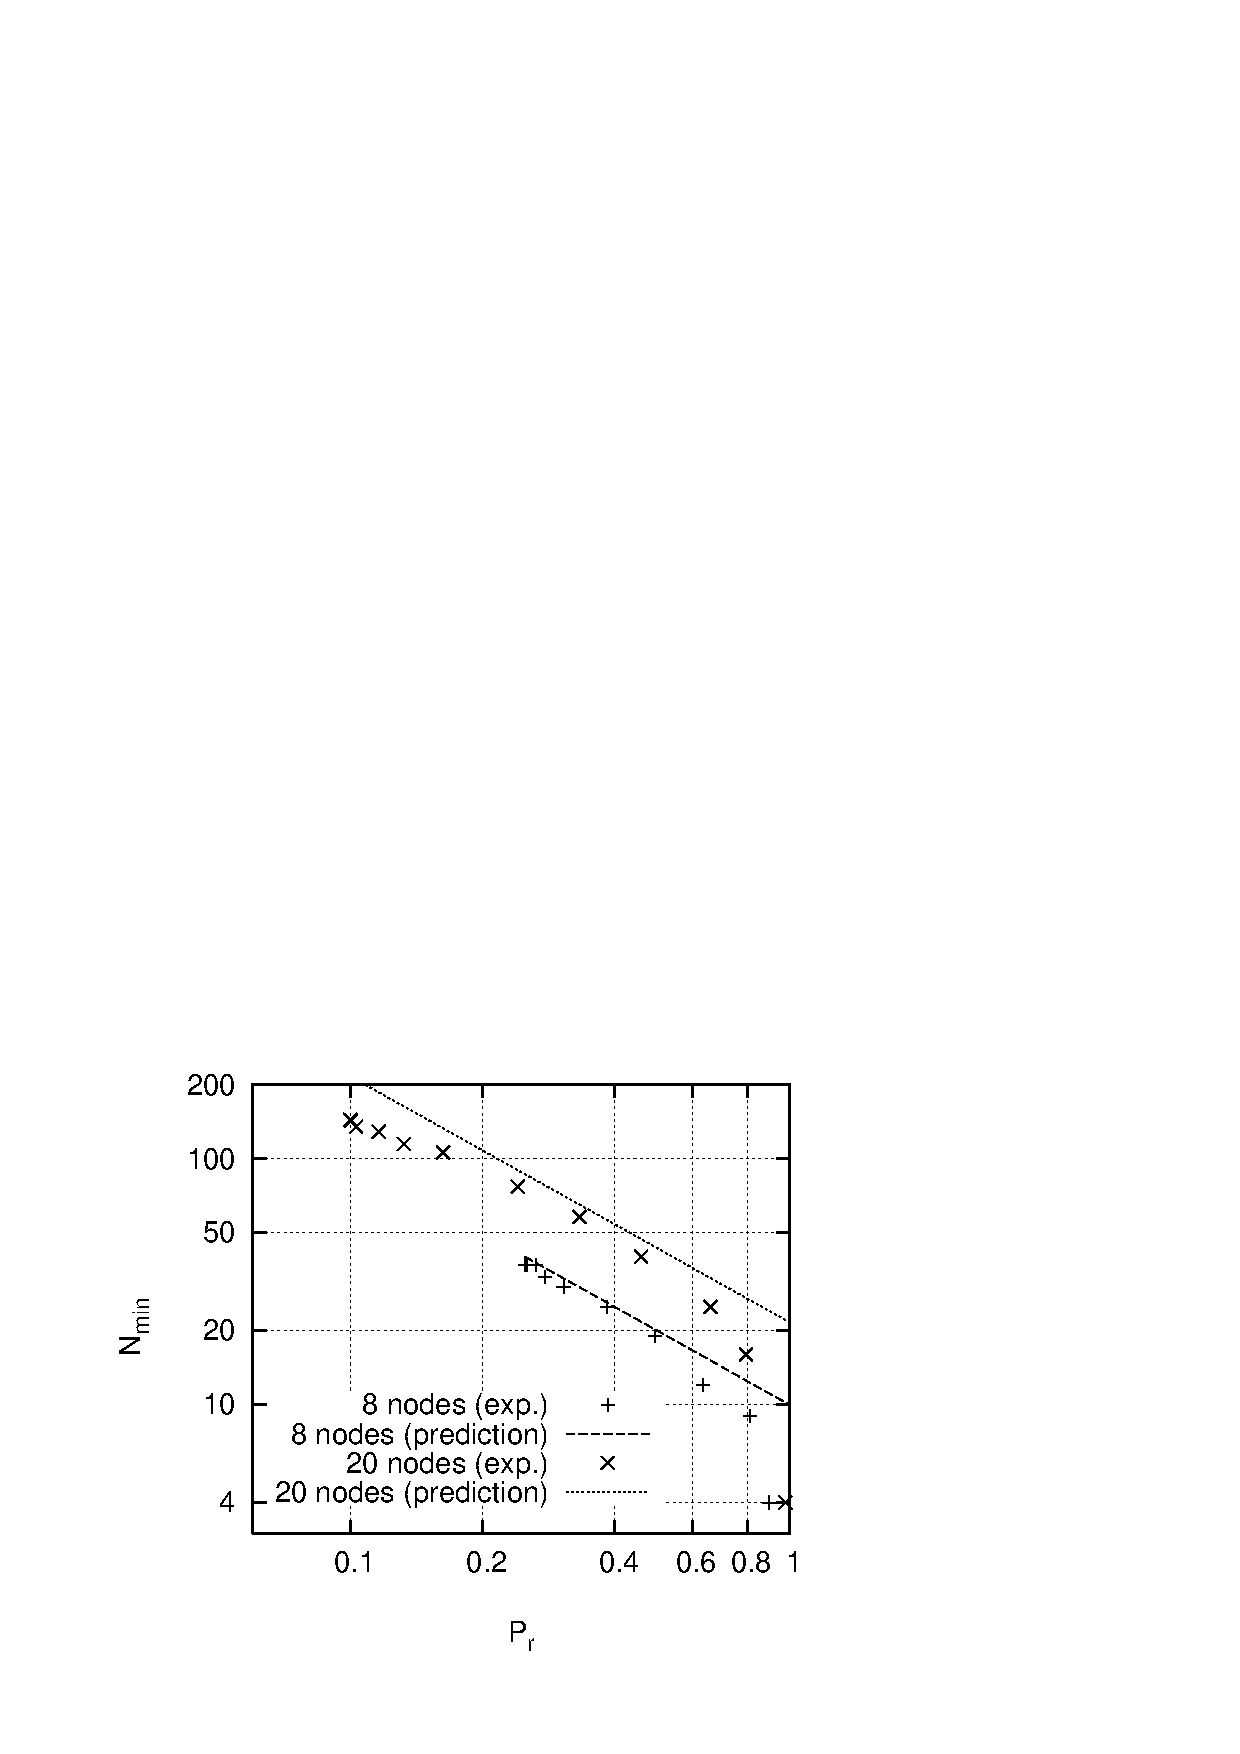
\includegraphics[width=\columnwidth]{grafiken/n-over-r8-20}
        }
\subfigure[Ein mit xfig erzeugtes Bild\label{fig:bild2}]
        {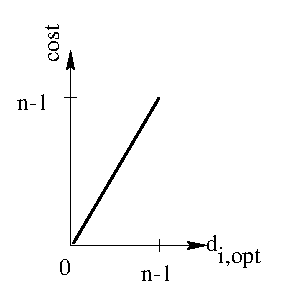
\includegraphics[width=3cm]{grafiken/cost}} 
\caption[Das hier steht im Abbildungsverzeichnis.]{Beispiele f{\"u}r sch{\"o}ne Bilder.\label{fig:bild1-und-bild2}}

\end{figure}


\section{Editor}

Als Editor f{\"u}r Fortgeschrittene ist xemacs gut geeignet.
Bei Verwendung von xemacs ist der Gebrauch der reftex und auctex-pakete zu empfehlen.
Als Rechtschreibprogramm sollte aspell verwendet werden und folgender Code in init.el eingef{\"u}gt werden.


 (require 'iso-cvt)\\
  (add-hook 'LaTeX-mode-hook\\
    (function (lambda ()\\
      ;; Setze Anfuehrungszeichen etc. fuer Style german\\
      (TeX-run-style-hooks "german")\\
      ;;\\
      ;; Lade Buffer und wandle nach ISO Latin-1:\\
      (format-encode-buffer 'plain)\\
      )))\\
\\
      (setq ispell-silently-savep t) ;save new words in pdict without questioning\\
(setq ispell-help-in-bufferp 'electric) ;get a better help buffer\\
(setq ispell-program-name "aspell")\\
(setq ispell-extra-args '("-W" "2"))\\
\\
(column-number-mode t)\\
\\
(custom-set-variables\\
 '(paren-mode 'sexp nil (paren)))\\
\\
 (setq reftex-plug-into-AUCTeX t)\\
(require 'reftex "reftex" t)\\
 (turn-on-reftex) ; use reftex\\
\\
 


Neulinge k{\"o}nnen auch einen sonstigen Editor oder Sachen wie Texnic Center, etc verwenden.

\section{Mathematik}

In latex kann man Formeln wundersch{\"o}n setzen.

\selectlanguage{english} % The following chapter is in english
As the following stuff is in English, we must change the hyphenation style.


The OCST problem is defined as follows. Let $G=(V,E)$ be a connected, undirected graph with $n=|V|$ nodes and $m=|E|$ edges. There are  communication, or transportation demands, between every pair of nodes.  An $n \times n$ {\em demand matrix} $R=(r_{ij})$ specifies the demands, where $r_{ij}$ is the amount of traffic required between location $v_i$ and $v_j$. Similarly, an $n\times n$ {\em distance matrix} $W=w_{ij}$ determines the distance weights between each pair of sites. 
A tree $T=(V,F)$ where $F \subseteq E$ and $|F|=|V|-1$ is called a {\em spanning tree} of $G$ if it connects all the nodes. The weight $w(T)$ of the spanning tree is the weighted sum over all pairs of vertices of the cost of the path between the pair in $T$. The communication cost over the tree $T$ is defined as 
\begin{equation}
  \label{equ:1}
w(T)=\sum_{i,j\in V}w_{ij}b_{ij},
\end{equation}
where $B=b_{ij}$ denotes the traffic flowing directly and indirectly across the edge connecting nodes $i$ and $j$. It is calculated according to the structure of $T$. 
$T$ is the optimal communication spanning tree if $w(T)\leq w(T')$ for all other spanning trees $T'$. %For the experiments we assume that there is an unique optimum tree ($w_{ij}\neq w_{kl}\forall (i\neq k, j\neq l)$).
The OCST problem becomes the minimum spanning tree (MST) problem if $w(T)=\sum_{i,j\in V}w_{ij}$. Then, $T$ is the simple minimum spanning tree if $w(T)\leq w(T')$  for all other spanning trees $T'$.%, where $w(T)=\sum_{i,j\in V}w_{ij}$. 
%In most instances of the OCST problem, the cost $f(w_{ij},b_{ij})$ of each link connecting the nodes $i$ and $j$ is calculated as the product of the distances $w_{ij}$ times the overall traffic $b_{ij}$ running over the link, so that $f=w_{ij}b_{ij}$. 

Cayley's formula identifies the number of spanning trees on $n$ nodes as $n^{n-2}$ . Furthermore, there are $n$ different stars on a graph of $n$ nodes. The similarity between two spanning trees $T_i$ and $T_j$ can be measured using the distance   $d_{ij}\in\{0,1,\ldots,n-1\}$ as 
$$
d_{ij}=\frac{1}{2}\sum_{u,v\in V,u<v}|l^{i}_{uv}-l^{j}_{uv}|,
$$
where $l^{i}_{uv}$ is 1 if an edge from $u$ to $v$ exists in $T_i$ and 0 if it does not exist in $T_i$. The number of edges that two trees $T_i$ and $T_j$ have in common is $n-1-d_{ij}$.




\selectlanguage{ngerman} % deutsch

Ab jetzt wieder deutsche Trennung.

In Abbildung \ref{fig:2dnorm} gibt es noch ein Beispiel f{\"u}r ein Bild und in Tabelle \ref{tab:einfache-tabelle} gibt es ein einfaches Bild. Tabelle~\ref{tab8:results-testproblem-deceptive} stellt eine etwas kompliziertere Tabelle dar. 
\begin{figure}[htb]
        \begin{center}
        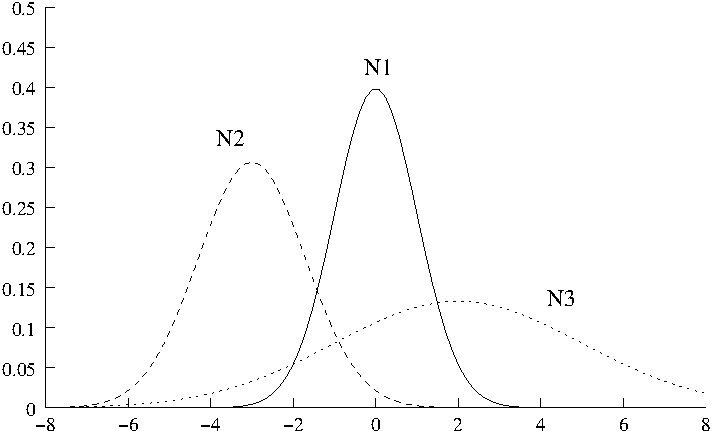
\includegraphics[width=8cm]{grafiken/norm_uni}
        \caption{Dichten univariater Normalverteilungen}
        \label{fig:2dnorm}
        \end{center}
\end{figure}


Beim Aufbau von Kommunikationsnetzen stehen Unternehmen vor dem Problem, eine Menge von unterschiedlichen Standorten so durch Leitungen zu verbinden, dass bestimmte Qualit{\"a}tsanforderungen (z.B. Sicherheit, Bandbreite, Zu\-ver\-l{\"a}ssig\-keit, Skalierbarkeit, etc.) eingehalten werden und gleichzeitig die Netzstruktur so gew{\"a}hlt wird, dass die Kosten des Netzaufbaus minimiert werden. Unternehmen, f{\"u}r welche der Aufbau von Kommunikationsnetzwerken relevant ist, lassen sich in zwei Gruppen unterteilen:

Auf der einen Seite sind Unternehmen zu finden, f{\"u}r die Kommunikationsnetzwerke ein wichtiger Teil ihrer Unternehmensinfrastruktur sind (z.B. Banken, Verlagsh{\"a}user, Bahn, Bundeswehr, Unternehmen mit mehreren Niederlassungen, etc.) und welche daher die Kommunikationsnetzwerke oft selbst betreiben. Ein Beispiel hierf{\"u}r ist die DATEV eG, welche {\"u}ber ein eigenes \glqq Genossenschaftsnetz'' mehrere Dutzend Niederlassungen an die Zentrale in N{\"u}rnberg anbindet. {\"U}ber dieses Kommunikationsnetz wird sowohl der gesamte Daten- als auch Telefonverkehr innerhalb des Unternehmens abgewickelt.


Auf der anderen Seite stehen Unternehmen, f{\"u}r die der Aufbau und der Betrieb von Kommunikationsnetzwerken Kernaufgaben darstellen (z.B. Telekommunikationsunternehmen (Deutsche Telekom oder Deutsches Forschungsnetz (DFN)), Mobilfunkbetreiber (vodafon, T-mobil) oder lokale Provider (NetCologne, Stadtwerke). F{\"u}r derartige Unternehmen geh{\"o}rt der Aufbau und Betrieb von Kommunikationsnetzwerken zum Kerngesch{\"a}ft. Netzwerke sind so aufzubauen und weiterzuentwickeln, dass Qualit{\"a}tskriterien eingehalten werden und gleichzeitig die Betriebskosten minimiert werden. 





\begin{table}
\caption{Eine sehr einfache Tabelle\label{tab:einfache-tabelle}}
\begin{center}
\begin{tabular}{|l|c|r|}
\hline
linksb{\"u}ndig & zentriert & rechtsb{\"u}ndig \\
\hline
1 & 2 & 3,141\\
\hline
\end{tabular}
\end{center}
\end{table}

Beim Aufbau von Kommunikationsnetzwerken kann unterschieden werden zwischen vermaschten und baumf{\"o}rmigen Netzwerken (vergleiche Abbildung \ref{fig:2dnorm}). In  vermaschten Netzen existieren mehrere unterschiedliche Wege f{\"u}r den Transport von Daten zwischen zwei Standorten. Daher muss bei vermaschten Netzwerken das Routing der Daten durch das Netzwerk gesteuert werden (wie z.B. im Internet). In der Regel existieren mehrere Wege zwischen zwei Standorten und es muss mit Hilfe von Routingmechanismen festgelegt werden, welchen Weg die Daten durch das Netz nehmen sollen (wie z.B. durch Routingtabellen f{\"u}r den IP-Verkehr im Internet). Diese Entscheidung wird unter anderem durch die Entfernung von Standorten als auch durch die Auslastung der unterschiedlichen Leitungen beeinflusst. Die Ermittlung von Routingtabellen ist in der Praxis recht aufwendig und es besteht die Gefahr, dass Nachrichten Umwege durch das Netz nehmen oder sogar im Kreis laufen. Vermaschte Netzwerke bieten allerdings eine erh{\"o}hte Ausfallsicherheit, da beim Vorhandensein von mehreren Wegen zwischen zwei Knoten Daten auch dann noch ausgetauscht werden k{\"o}nnen, wenn ein Teil des Netzwerkes ausf{\"a}llt.



\begin{table}
\centering
\caption{Performance of GAs using different types of representations for deceptive tree problems of different sizes and with different $T_{opt}$ (arbitrary tree, MST, and star)\label{tab8:results-testproblem-deceptive}}

\begin{tabular}{c|l|c|cc|cc}

\multirow{3}{*}{\rotatebox{90}{$T_{opt}$}}  && \multicolumn{5}{c}{oder 3}\\ \cline{3-7}
 && \multirow{2}{*}{$P_{succ}$}& \multicolumn{2}{c|}{fitness}& \multicolumn{2}{c}{$t_{conv}$}\\
& & &$\mu$ & $\sigma$& $\mu$ & $\sigma$  \\ \noalign{\vskip\arrayrulewidth\hrule height 1pt}
%
\multirow{7}{*}{\rotatebox{90}{arbitrary tree}} & Pr{\"u}fer number & 0.54 & 0.49 & (0.6) & 26.0 & (8.6 \\ \cline{2-7}
 & NetKey & 0.78 & 0.23 & (0.4) & 23.0 & (6.0) \\ \cline{2-7}
 & LB ($P_1$=1)  & 0.09 & 1.69 & (0.8) & 19.5 & (7.6) \\
 & LB ($P_1$=20) & 0.82 & 0.18 & (0.4) & 23.3 & (6.1)  \\
 & $P_1$=$P_2$=1 & 0.12 & 1.24 & (0.6) & 27.4 & (8.0) \\ \cline{2-7}
 & heur. xover & 0 & 2.63 & (0.5) & 8.7 & (2.4)   \\
 & h. ini \& xover  & 0 & 3.88 & (0.1) & 0.4 & (0.4) \\
\end{tabular}
\end{table}


Baumf{\"o}rmige Netze stellen einen Sonderfall von vermaschten Kommunikationsnetzwerken dar. Hierbei existiert genau ein m{\"o}glicher Weg zwischen den Knoten im Netz. Daher muss keine Entscheidung {\"u}ber das Routing getroffen werden und Routingmechanismen zur Steuerung des Datenflusses entfallen. Allerdings haben baumf{\"o}rmige Netzwerke das Problem, dass durch den Ausfall einer Leitung ein Teil der Knoten nicht mehr erreichbar sind. Baumf{\"o}rmige Kommunikationsnetzwerke werden oft bei einer {\"u}berschaubaren Anzahl von Standorten wie z.B. in Local Area Networks (LAN) oder Unternehmensnetzwerken (\glqq Corporate Networks'') eingesetzt. Insbesondere Unternehmen, welche eigene Netzwerke betreiben (z.B. die DATEV eG), verwenden oft baum\-f{\"o}r\-mi\-ge Kommunikationsnetzwerkstrukturen wegen ihrer geringereren Komplexit{\"a}t. 

Das Problem des kostenminimalen Aufbaus von vermaschten bzw. baumf{\"o}rmigen Kommunikationsnetzen wurde schon sehr fr{\"u}hzeitig in der Literatur formalisiert und beschrieben. Beim \glqq network design problem'' soll diejenige Netzwerkstruktur bestimmt werden, welche alle Standorte miteinander verbindet, alle Kommunikationsanforderungen zwischen den einzelnen Standorten erf{\"u}llt und gleichzeitig minimale Kosten besitzt. Aus dem allgemeinen \glqq network design problem'' l{\"a}sst sich das \glqq optimal communication spanning tree'' (OCST)-Problem ableiten, bei welchem die Struktur des gew{\"u}nschten Netzwerkes baumf{\"o}rmig ist. Im folgenden Abschnitt soll n{\"a}her auf das OCST Problem eingegangen werden.



%%% Local Variables: 
%%% mode: latex
%%% TeX-master: "..\\da-beispiel"
%%% End: 

%\chapter{Discussion, Conclusions, and Further Work}
\label{chap:conclusions}
The purpose of this book is to understand  the influence of representations on the performance of genetic and evolutionary algorithms. 
This chapter summarizes the work contained in this study and lists its major contributions.


\section{Discussion}
\label{sec:discussion}

This is the final section \ref{sec:summary}. We  started in Chap.~\ref{chap:howto} by providing the necessary background for examining representations for  GEAs. Researchers recognized early that representations have a large influence on the performance of GEAs. Consequently, after a brief introduction into representations and GEAs, we discussed how the influence of representations on problem difficulty  can be measured. The chapter ended with prior guidelines for choosing high-quality  representations. Most of them are  mainly based on empirical observations and intuition and not on theoretical analysis.

Therefore, we presented in Chap.~\ref{cha:grafiken} three aspects of a theory of representations for  GEAs. We investigated how the locality, scaling, and locality of an encoding  influences GEA performance. The performance of GEAs is determined by the solution quality at the end of a run and the number of generations until the population is converged. Consequently, for redundant and exponentially scaled encodings, we presented population sizing models and described how the time to convergence is changed.
Furthermore, we were able to demonstrate that high-locality encodings do not change the difficulty of a problem; in contrast, when using low-locality encodings, on average, the difficulty of problems changes. Therefore,  easy problems become more difficult and difficult problems become easier by the use of low-locality encodings.
For all three properties of encodings, the theoretical models were verified with empirical results.


\section{Conclusions}
We  summarize the most important contributions of this work.

{\bf Framework for design and analysis of representations (and operators) for GEAs.} The main purpose of this study was to present a  framework which describes how genetic representations influence the performance of GEAs. The performance of GEAs is measured by the solution quality at the end of the run and the number of generations until the population is converged. 
The proposed framework allows us to analyze the influence of existing representations on GEA performance and to develop efficient new representations in a theory-guided way.
Furthermore, we illustrated that the framework can also be used for the design and analysis of search operators, which are relevant for direct encodings.
Based on the framework, the development of high-quality representations remains not only a matter of intuition and random search but becomes an engineering design task.
Even though more work is needed, we believe that the results presented are sufficiently compelling to recommend increased use of the framework.



{\bf Redundancy, Scaling, and Locality}. These are the three elements of the proposed framework of representations.  We demonstrated that these three properties of representations influence GEA performance and presented theoretical models to predict how solution quality and time to convergence changes.
By examining the redundancy, scaling, and locality of an encoding, we are able to predict the influence of representations on GEA performance.

The theoretical analysis shows that the redundancy of an encoding influences the supply of building blocks (BB) in the initial population. $r$ denotes the number of genotypic BBs that represent the best phenotypic BB, and $k_r$ denotes the order of redundancy. For synonymously redundant encodings, where all genotypes that represent the same phenotype are similar to each other, the probability of GEA failure goes either with  $O(\exp(-r/2^{k_r}))$ (uniformly scaled representations) or  with $O(\exp(-\sqrt{r/2^{k_r}}))$ (exponentially scaled representations).
Therefore, GEA performance increases if the representation overrepresents high-quality BBs. If a representation is uniformly redundant, that means each phenotype is represented by the same number of genotypes, GEA performance remains unchanged in comparison to non-redundant encodings.

The analysis of the scaling of an encoding reveals that non-uniformly scaled representations modify the dynamics of genetic search. If exponentially scaled representations are used, the alleles are solved serially which increases the overall time until convergence and results in problems with genetic drift but allows rough approximations of the expected optimal solution after a few generations.

We know from previous work that the high locality of an encoding is a necessary condition for efficient mutation-based search.
An encoding has high locality if neighboring phenotypes correspond to neighboring genotypes.
Investigating the  influence of locality shows that  high-locality encodings do not change the difficulty of a problem. In contrast, low-locality encodings, where phenotypic neighbors do not correspond to genotypic neighbors, change problem difficulty and make, on average, easy problems more difficult and deceptive problems easier.
Therefore, to assure that  an easy problem remains easy, high-locality representations  are necessary.

\section{Further Work}

What are the open questions? What should be done next?




%%% Local Variables: 
%%% mode: latex
%%% TeX-master: "..\\da-beispiel"
%%% End: 

%\selectlanguage{ngerman} % wenn im Inhaltsverzeichnis Appendix stehen soll, muss Engl gewaehlt sein, fuer Anhang Deutsch
\appendix

%Bibliographie
%waehle einen der folgenden 4 Eintraege
%\bibliographystyle{literatur/natdin} %DIN Style Literaturverzeichnis, comment out pagebackref
%\bibliographystyle{literatur/IEEEtran} % IEEE Style Literaturverzeichnis
%\bibliographystyle{literatur/natdinCustomized} %DIN Style Literaturverzeichnis + Punkt hinter jeder Literaturangabe -> low level config fuer Zitate: natdin.cfg im Projektordner, comment out pagebackref
%\bibliographystyle{literatur/natdinCustomizedEnglish} %DIN Style auf Englisch getrimmt mit Punkt hinter Literaturangabe -> low lovel config fuer Zitate: natdin.cfg im Projektordner, pagebackref kann damit nicht genutzt werden
%\bibliographystyle{aer} % alternativ auch apalike, aer, apalike2... s.a. http://web.reed.edu/cis/Help/LaTeX/bibtexstyles.html
\bibliographystyle{plainnat} % very nice bib style
%note on aer: does not like inbook entries
%\bibliographystyle{natdin}

\bibliography{literatur/lit} %Pfad zur bib-Datei

%appendices can be defined here, the appendix structure has to be added manually to the toc (table of contents)
%\clearpage  %toc new page
%\addcontentsline{toc}{chapter}{Appendix} %add chapter to toc
\addpart{\appendixname}
\chapter{Simile - Code}
\label{append:simile-code}
In this section we will expose the different Java classes of our prototype.

\section{de.unimannheim.informatik.swt.simile}
\lstinputlisting[
  language=Java, numbers=left, stepnumber=5, firstnumber=1, breaklines=true, 
  basicstyle=\footnotesize,
  numberstyle=\tiny,
  caption={Simile.java},
  captionpos=b,
  label=Simile.java
]
{code/main/Simile.java.txt}

\lstinputlisting[
  language=Java, numbers=left, stepnumber=5, firstnumber=1, breaklines=true, 
  basicstyle=\footnotesize,
  numberstyle=\tiny,
  caption={ServletInitializer.java},
  captionpos=b,
  label=ServletInitializer.java
]
{code/main/ServletInitializer.java.txt}

\lstinputlisting[
  language=Java, numbers=left, stepnumber=5, firstnumber=1, breaklines=true, 
  basicstyle=\footnotesize,
  numberstyle=\tiny,
  caption={SimileApplication.java},
  captionpos=b,
  label=SimileApplication.java
]
{code/main/SimileApplication.java.txt}
\subsection{de.unimannheim.informatik.swt.simile.controllers}
\lstinputlisting[
  language=Java, numbers=left, stepnumber=5, firstnumber=1, breaklines=true, 
  basicstyle=\footnotesize,
  numberstyle=\tiny,
  caption={EntryController.java},
  captionpos=b,
  label=EntryController.java
]
{code/controller/EntryController.java.txt}
\subsection{de.unimannheim.informatik.swt.simile.model}
\lstinputlisting[
  language=Java, numbers=left, stepnumber=5, firstnumber=1, breaklines=true, 
  basicstyle=\footnotesize,
  numberstyle=\tiny,
  caption={Candidate.java},
  captionpos=b,
  label=Candidate.java
]
{code/model/Candidate.java.txt}

\lstinputlisting[
  language=Java, numbers=left, stepnumber=5, firstnumber=1, breaklines=true, 
  basicstyle=\footnotesize,
  numberstyle=\tiny,
  caption={Message.java},
  captionpos=b,
  label=Message.java
]
{code/model/Message.java.txt}

\lstinputlisting[
  language=Java, numbers=left, stepnumber=5, firstnumber=1, breaklines=true, 
  basicstyle=\footnotesize,
  numberstyle=\tiny,
  caption={Metric.java},
  captionpos=b,
  label=Metric.java
]
{code/model/Metric.java.txt}
\subsection{de.unimannheim.informatik.swt.simile.services}
\lstinputlisting[
  language=Java, numbers=left, stepnumber=5, firstnumber=1, breaklines=true, 
  basicstyle=\footnotesize,
  numberstyle=\tiny,
  caption={Cloner.java},
  captionpos=b,
  label=Cloner.java
]
{code/services/Cloner.java.txt}

\lstinputlisting[
  language=Java, numbers=left, stepnumber=5, firstnumber=1, breaklines=true, 
  basicstyle=\footnotesize,
  numberstyle=\tiny,
  caption={DirectoryExplorer.java},
  captionpos=b,
  label=DirectoryExplorer.java
]
{code/services/DirectoryExplorer.java.txt}

\lstinputlisting[
  language=Java, numbers=left, stepnumber=5, firstnumber=1, breaklines=true, 
  basicstyle=\footnotesize,
  numberstyle=\tiny,
  caption={EmailSender.java},
  captionpos=b,
  label=EmailSender.java
]
{code/services/EmailSender.java.txt}

\lstinputlisting[
  language=Java, numbers=left, stepnumber=5, firstnumber=1, breaklines=true, 
  basicstyle=\footnotesize,
  numberstyle=\tiny,
  caption={FileHandler.java},
  captionpos=b,
  label=FileHandler.java
]
{code/services/FileHandler.java.txt}

\lstinputlisting[
  language=Java, numbers=left, stepnumber=5, firstnumber=1, breaklines=true, 
  basicstyle=\footnotesize,
  numberstyle=\tiny,
  caption={Filter.java},
  captionpos=b,
  label=Filter.java
]
{code/services/Filter.java.txt}

\lstinputlisting[
  language=Java, numbers=left, stepnumber=5, firstnumber=1, breaklines=true, 
  basicstyle=\footnotesize,
  numberstyle=\tiny,
  caption={JavaClassFilter.java},
  captionpos=b,
  label=JavaClassFilter.java
]
{code/services/JavaClassFilter.java.txt}

\lstinputlisting[
  language=Java, numbers=left, stepnumber=5, firstnumber=1, breaklines=true, 
  basicstyle=\footnotesize,
  numberstyle=\tiny,
  caption={JavaClassHandler.java},
  captionpos=b,
  label=JavaClassHandler.java
]
{code/services/JavaClassHandler.java.txt}

\lstinputlisting[
  language=Java, numbers=left, stepnumber=5, firstnumber=1, breaklines=true, 
  basicstyle=\footnotesize,
  numberstyle=\tiny,
  caption={JavaClassVisitor.java},
  captionpos=b,
  label=JavaClassVisitor.java
]
{code/services/JavaClassVisitor.java.txt}

\lstinputlisting[
  language=Java, numbers=left, stepnumber=5, firstnumber=1, breaklines=true, 
  basicstyle=\footnotesize,
  numberstyle=\tiny,
  caption={JavaMethodVisitor.java},
  captionpos=b,
  label=JavaMethodVisitor.java
]
{code/services/JavaMethodVisitor.java.txt}

\lstinputlisting[
  language=Java, numbers=left, stepnumber=5, firstnumber=1, breaklines=true, 
  basicstyle=\footnotesize,
  numberstyle=\tiny,
  caption={NodeIterator.java},
  captionpos=b,
  label=NodeIterator.java
]
{code/services/NodeIterator.java.txt}

\lstinputlisting[
  language=Java, numbers=left, stepnumber=5, firstnumber=1, breaklines=true, 
  basicstyle=\footnotesize,
  numberstyle=\tiny,
  caption={SocoraRequester.java},
  captionpos=b,
  label=SocoraRequester.java
]
{code/services/SocoraRequester.java.txt}
\subsection{de.unimannheim.informatik.swt.simile.util}
\lstinputlisting[
  language=Java, numbers=left, stepnumber=5, firstnumber=1, breaklines=true, 
  basicstyle=\footnotesize,
  numberstyle=\tiny,
  caption={StreamGobbler.java},
  captionpos=b,
  label=StreamGobbler.java
]
{code/util/StreamGobbler.java.txt}

\chapter{Installation of Simile}
In this chapter we will show how to install the tools we used for implementing Simile. First we will start installing the CI Server Jenkins and explain how to configure it. Then, we will continue with installing Simile Jenkins plugin. After that we will explain how to configure Simile Jenkins plugin using the test project.

\section{Installation of Jenkins}
In this section we will explain how to install Jenkins CI server using Docker.

\subsection{Docker}
For installing Jenkins, we will use Docker containers and in this subsection we will explain how to install it in different platform such as macOS and Linux.

\subsubsection{Docker on macOS}
For macOS we will use Docker for Mac tool. This is an integrated, easy-to-deploy environment for building, assembling, and shipping applications from a Mac. Moreover, it is a native Mac application architected from scratch, with a native user interface and auto-update capability, deeply integrated with OS X native virtualization, Hypervisor Framework, networking and file system, making it faster and more reliable than previous ways of getting Docker on a Mac \cite{Docker}.

First we will download the tool from the following link: \url{https://download.docker.com/mac/stable/Docker.dmg}.\\

After downloading the \textit{dmg} image, double-click on it and you will see something like figure \ref{fig:docker-mac-01}. When you get that image, drag and drop the Docker icon to the Applications folder. After that, go to Applications folder and double click on Docker application.

\begin{figure}[ht]
	\centering
    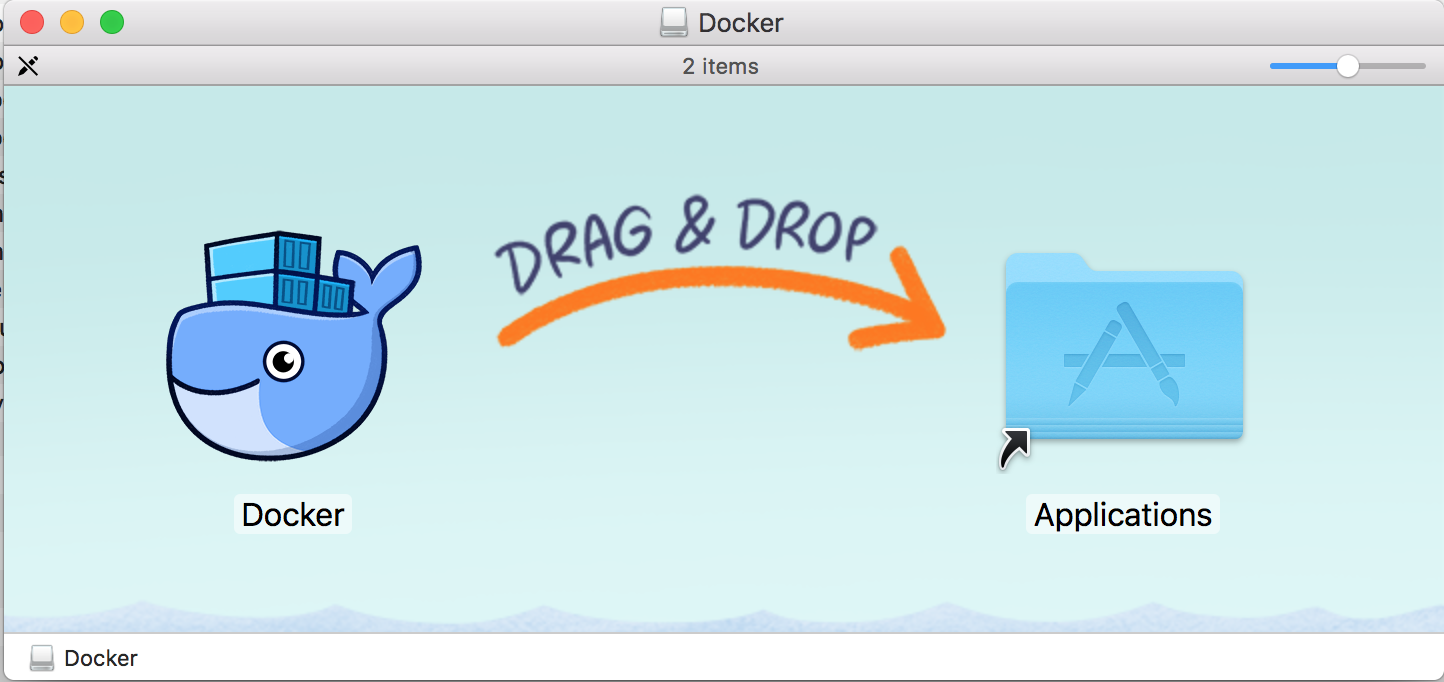
\includegraphics[width=\textwidth]{grafiken/docker-01}
    \caption{Docker for Mac installation}
    \label{fig:docker-mac-01}
\end{figure}

\subsubsection{Docker on Linux}
In this section we will explain how to install Docker in Linux, specifically in Debian (Jessie). For other distros please refer to Docker documentation\footnote{https://docs.docker.com/engine/installation/linux/ (accessed: 21.01.2017)}.

First of all we need to update the repositories.

\begin{minted}[linenos,
               numbersep=5pt,
               frame=lines,
               framesep=2mm]{bash}
$ sudo apt-get udpate
\end{minted}

Then we need to install the packages to allow \textit{apt} to use repositories iver HTTPS.

\begin{minted}[linenos,
               numbersep=5pt,
               frame=lines,
               framesep=2mm]{bash}
$ sudo apt-get install apt-transport-https \
                       ca-certificates \
                       software-properties-common
\end{minted}

Then we add the official Docker's GPG key.

\begin{minted}[linenos,
               numbersep=5pt,
               frame=lines,
               framesep=2mm]{bash}
$ curl -fsSL https://yum.dockerproject.org/gpg | sudo apt-key add -
\end{minted}

Finally we add the stable repository of Docker and update repositories.

\begin{minted}[linenos,
               numbersep=5pt,
               frame=lines,
               framesep=2mm]{bash}
$ sudo add-apt-repository \
       "deb https://apt.dockerproject.org/repo/ \
       debian-$(lsb_release -cs) \
       main"
$ sudo apt-get update
\end{minted}

Once we added the new repositories, we update the repository list.

\begin{minted}[linenos,
               numbersep=5pt,
               frame=lines,
               framesep=2mm]{bash}
$ sudo apt-get update
\end{minted}

Then we install docker.

\begin{minted}[linenos,
               numbersep=5pt,
               frame=lines,
               framesep=2mm]{bash}
$ sudo apt-get -y install docker-engine
\end{minted}

After the installation is done we can make a little test to be sure that everything was installed correctly. The following command will download a test image and runs it in a container. Once it is running will print an informational message and exits.

\begin{minted}[linenos,
               numbersep=5pt,
               frame=lines,
               framesep=2mm]{bash}
$ sudo docker run hello-world
\end{minted}

\subsection{Jenkins in Docker}
Open a terminal on your mac and enter the following command to download the Jenkins image for Docker.

\begin{minted}[linenos,
               numbersep=5pt,
               frame=lines,
               framesep=2mm]{bash}
$ docker pull jenkins
  Using default tag: latest
  latest: Pulling from library/jenkins

  # some irrelevant output was remove
  Digest: sha256:5046434030be395ec977c98e11...
  Status: Downloaded newer image for jenkins:latest
\end{minted}

Then, we just need to run the Jenkins image with the following command.

\begin{minted}[linenos,
               numbersep=5pt,
               frame=lines,
               framesep=2mm,
               breakanywhere]{bash}
$ docker run -p 8080:8080 -p 50000:50000 jenkins
  # some irrelevant output was remove
  *************************************************************

  Jenkins initial setup is required. An admin user has been 
  created and a password generated.
  Please use the following password to proceed to installation:

  95199411f1894bfa97e937147c41aa62 # IMPORTANT, default admin pass

  This may also be found at: /var/jenkins_home/secrets/initial.
 
  *************************************************************
  # some irrelevant output was removed
  Jan 19, 2017 8:28:05 AM hudson.model.AsyncPeriodicWork$1 run
  INFO: Finished Download metadata. 25,312 ms
\end{minted}

After that, open the following URL \url{http://localhost:8080} and you should see some like figure \ref{fig:jenkins-01}.

\begin{figure}[H]
	\centering
    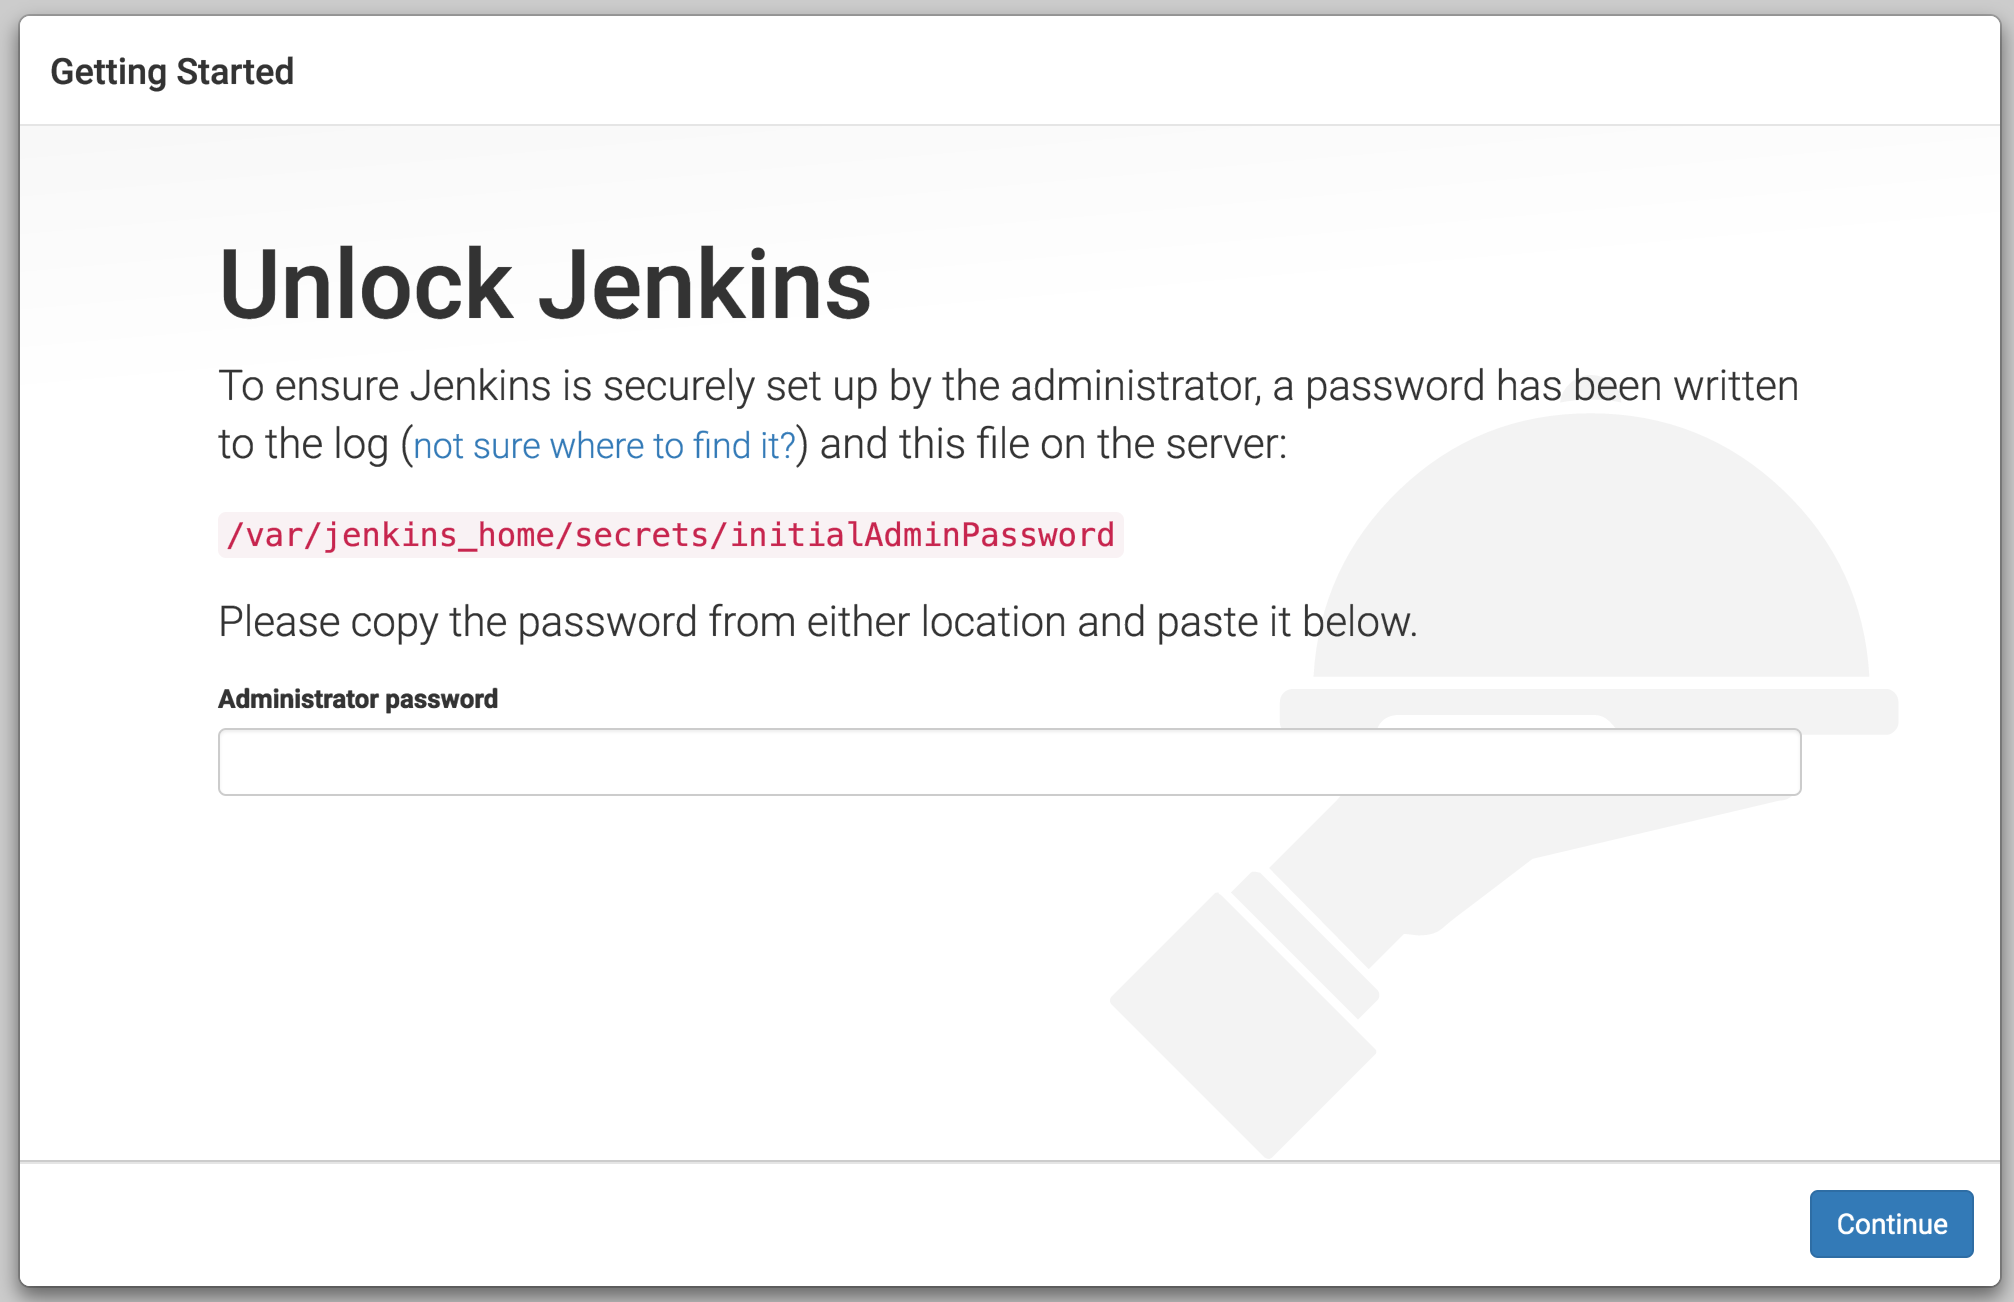
\includegraphics[width=0.7\textwidth]{grafiken/jenkins-01}
    \caption{First page of Jenkins setup}
    \label{fig:jenkins-01}
\end{figure}

There enter the password generated by Jenkins and that appeared in the logs, and then click on continue.

In the folowing page click on \textit{Install suggested plugins} like the figure \ref{fig:jenkins-02}.

\begin{figure}[H]
	\centering
    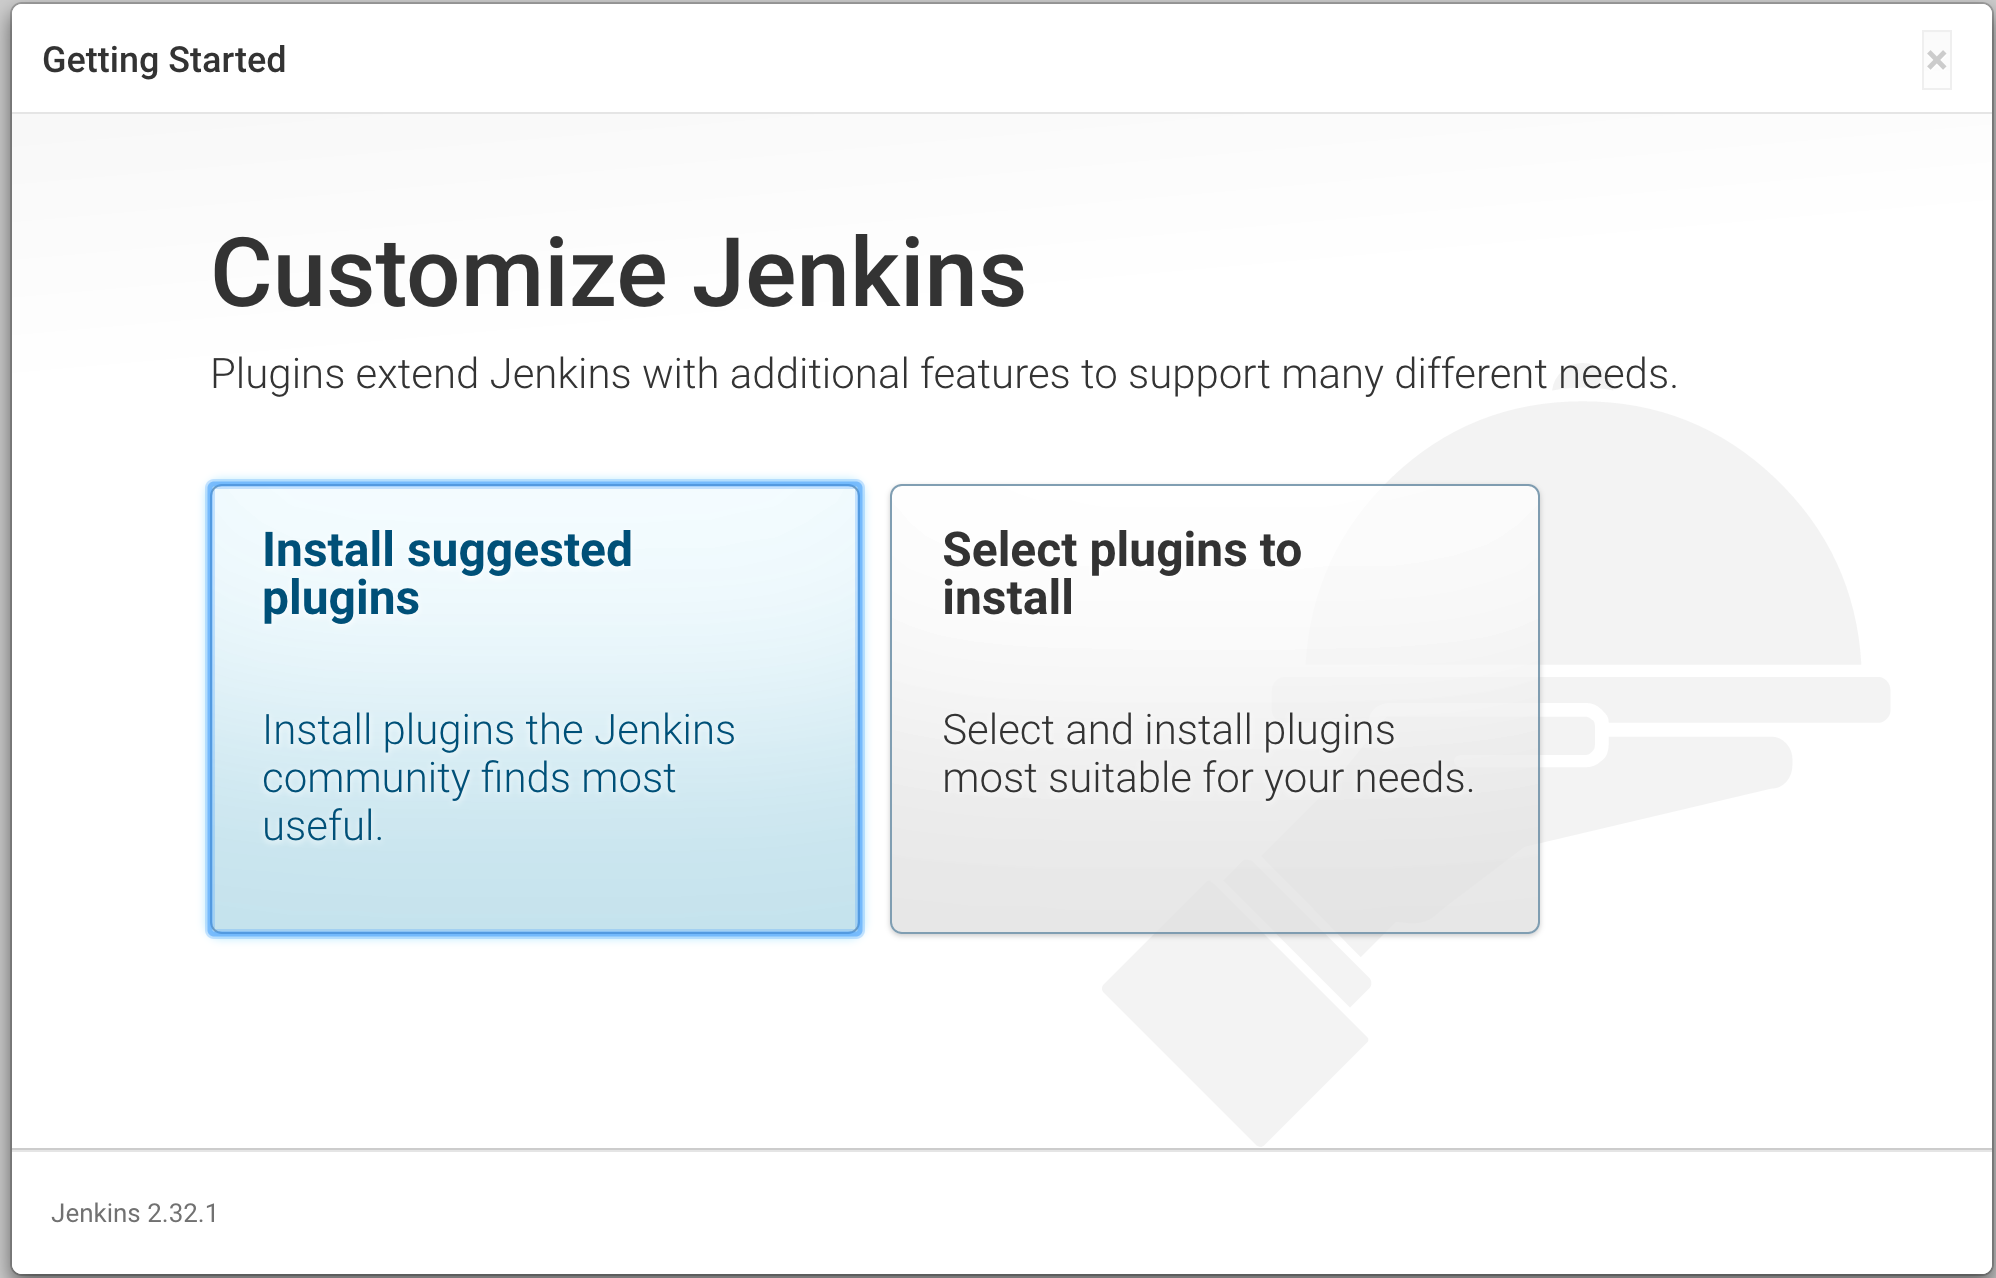
\includegraphics[width=0.8\textwidth]{grafiken/jenkins-02}
    \caption{Second page of Jenkins setup}
    \label{fig:jenkins-02}
\end{figure}

Then you should see something like the figure \ref{fig:jenkins-03}. Here we just need to wait untill the plugins installation finish.

\begin{figure}[H]
	\centering
    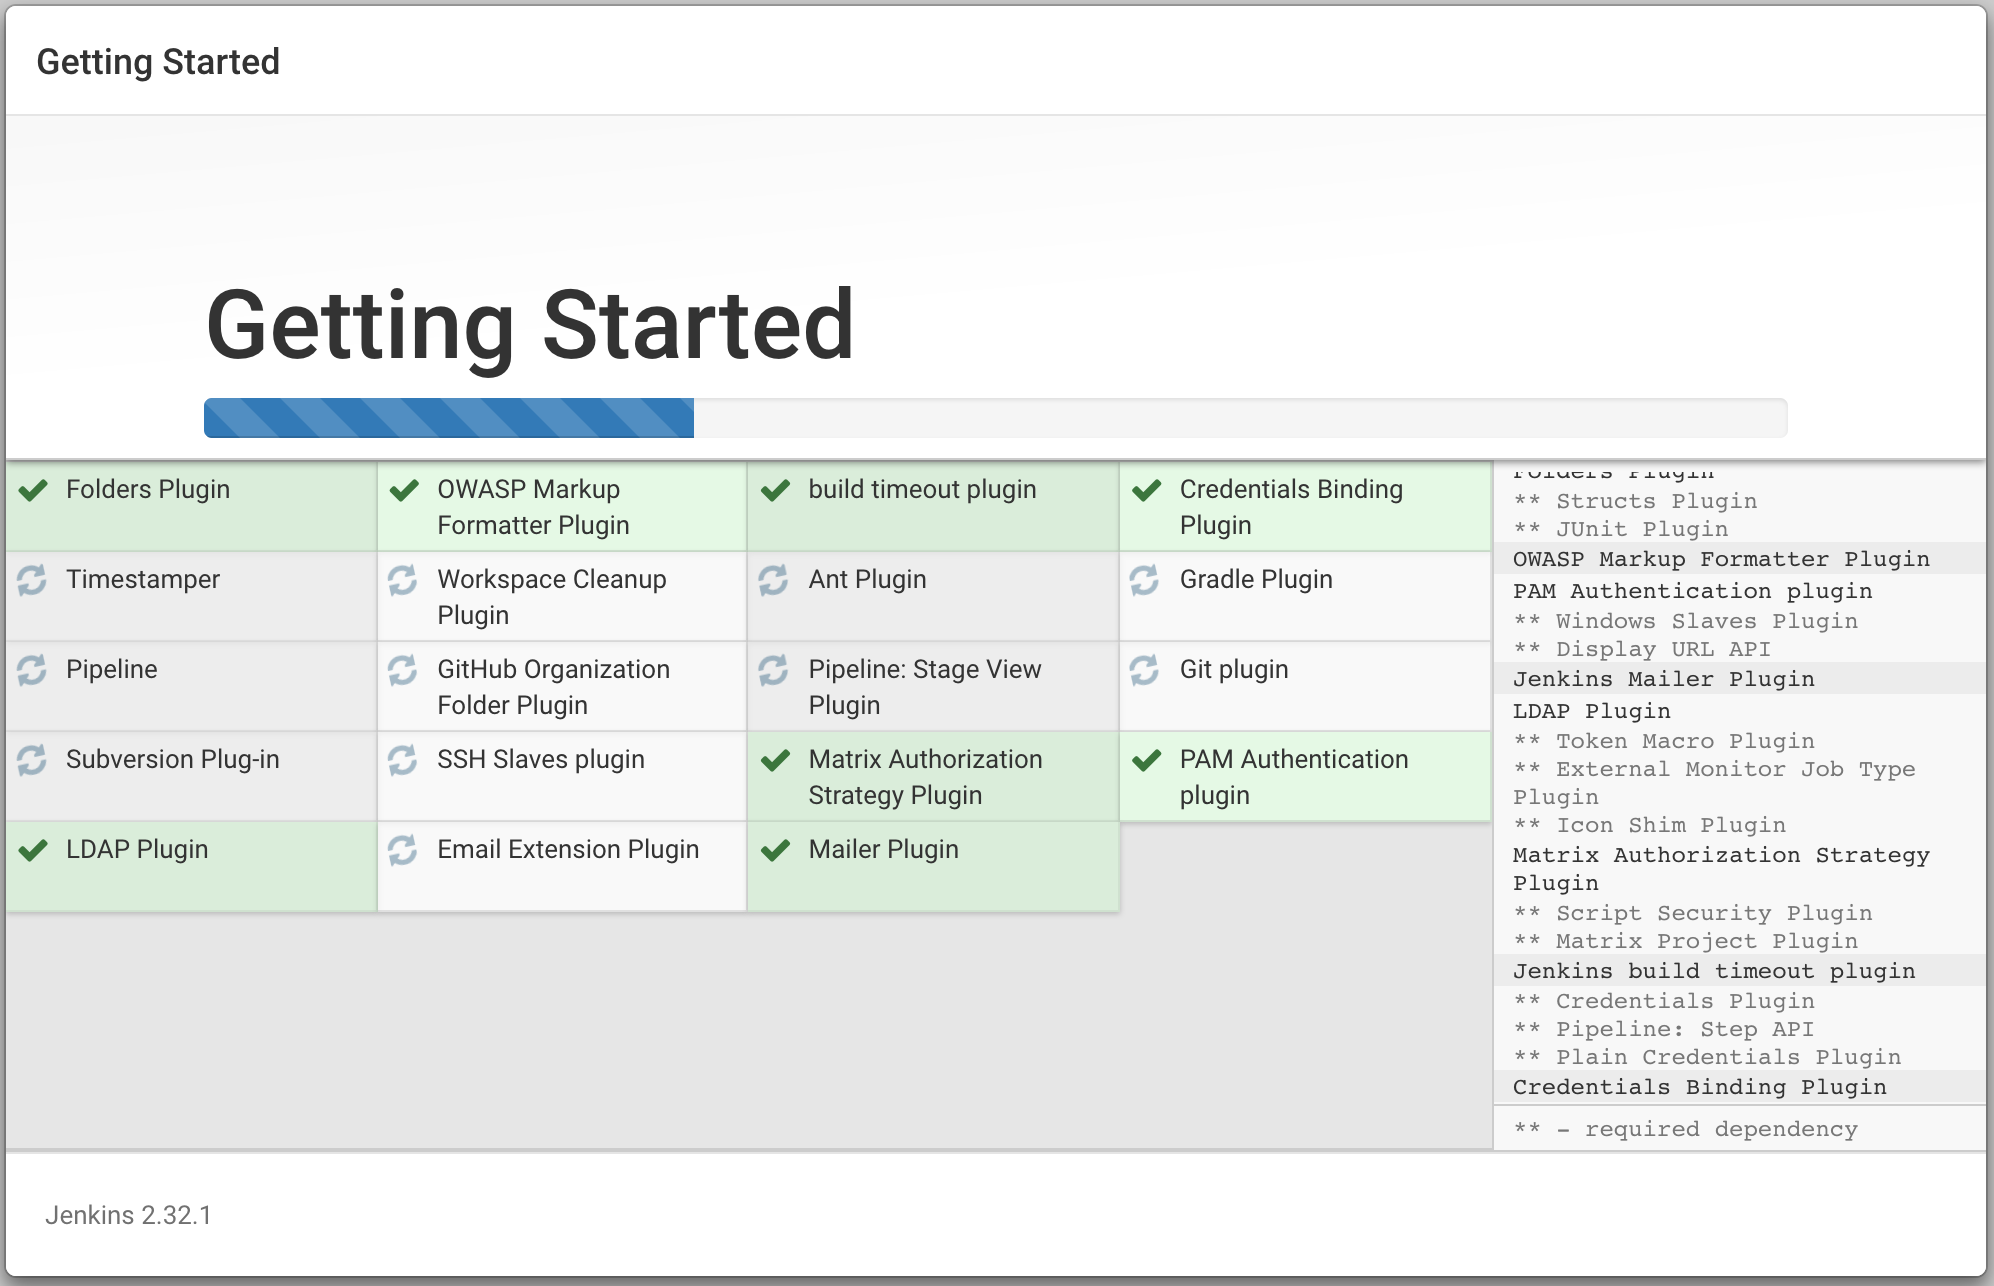
\includegraphics[width=0.8\textwidth]{grafiken/jenkins-03}
    \caption{Third page of Jenkins setup}
    \label{fig:jenkins-03}
\end{figure}

After the installation of plugins is done, click on \textit{Continue as admin} or create custom admin user. Then you should see the home page of Jenkins (figure )

\begin{figure}[H]
	\centering
    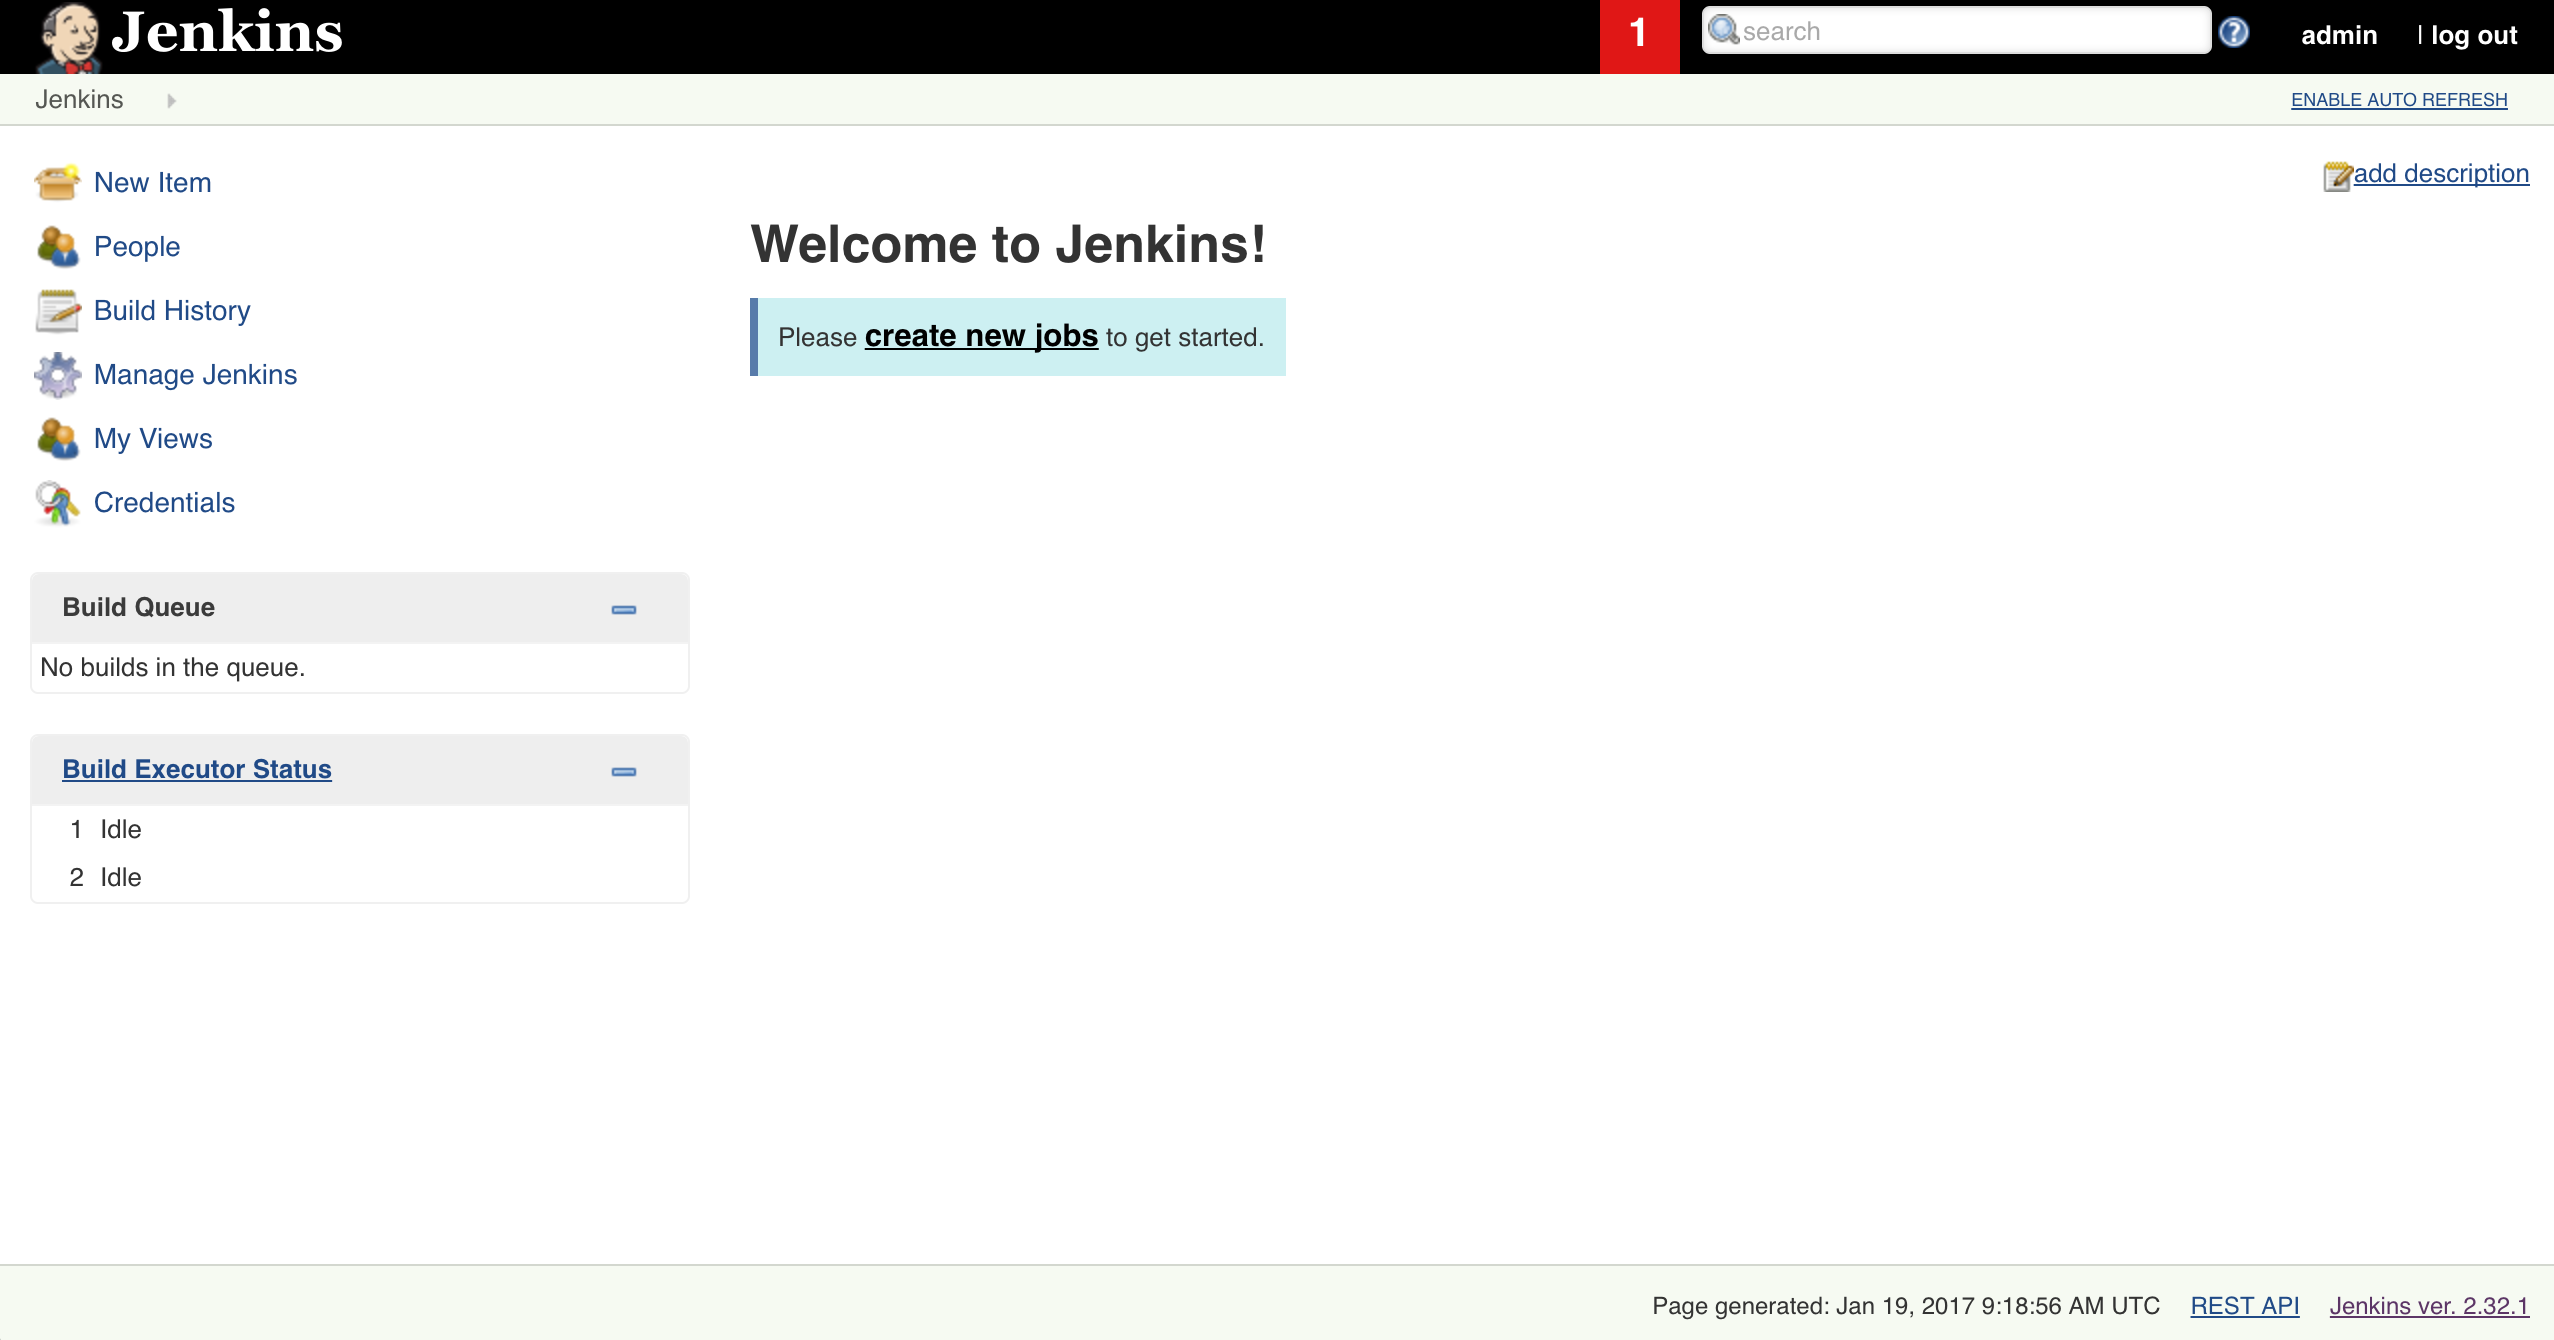
\includegraphics[width=0.8\textwidth]{grafiken/jenkins-04}
    \caption{Jenkins home page}
    \label{fig:jenkins-04}
\end{figure}

\section{Simile Jenkins Plugin installation}
To install Simile Jenkins plugin, we need to follow the following steps.

First, open Jenkins URL. Then click on \textit{Manage Jenkins} (figure \ref{fig:jenkins-plugin-01}).

\begin{figure}[H]
	\centering
    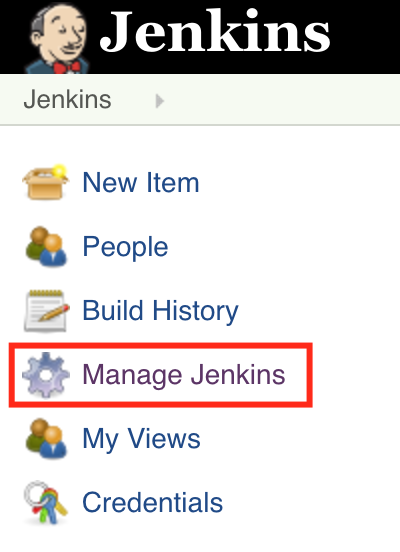
\includegraphics[width=0.25\textwidth]{grafiken/jenkins-plugin-01}
    \caption{Manage Jenkins option}
    \label{fig:jenkins-plugin-01}
\end{figure}

Then click on \textit{Manage Plugins} (figure \ref{fig:jenkins-plugin-02}).

\begin{figure}[H]
	\centering
    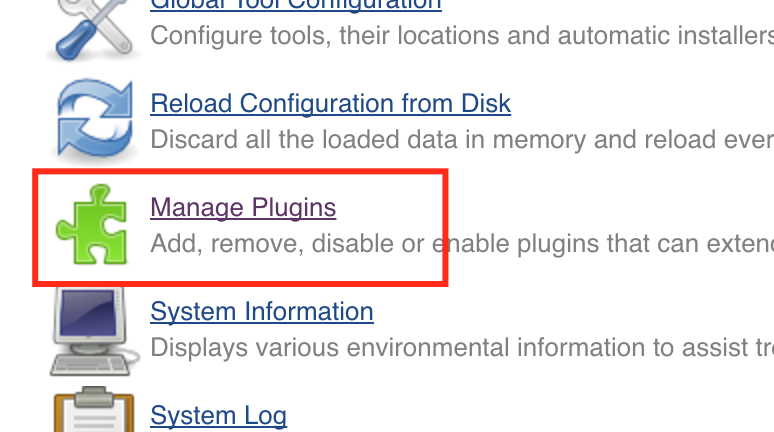
\includegraphics[width=0.5\textwidth]{grafiken/jenkins-plugin-02}
    \caption{Manage Plugins option}
    \label{fig:jenkins-plugin-02}
\end{figure}

Then go to \textit{Advanced}, scroll down until \textit{Upload Plugin} section (figure \ref{fig:jenkins-plugin-03}).

\begin{figure}[H]
	\centering
    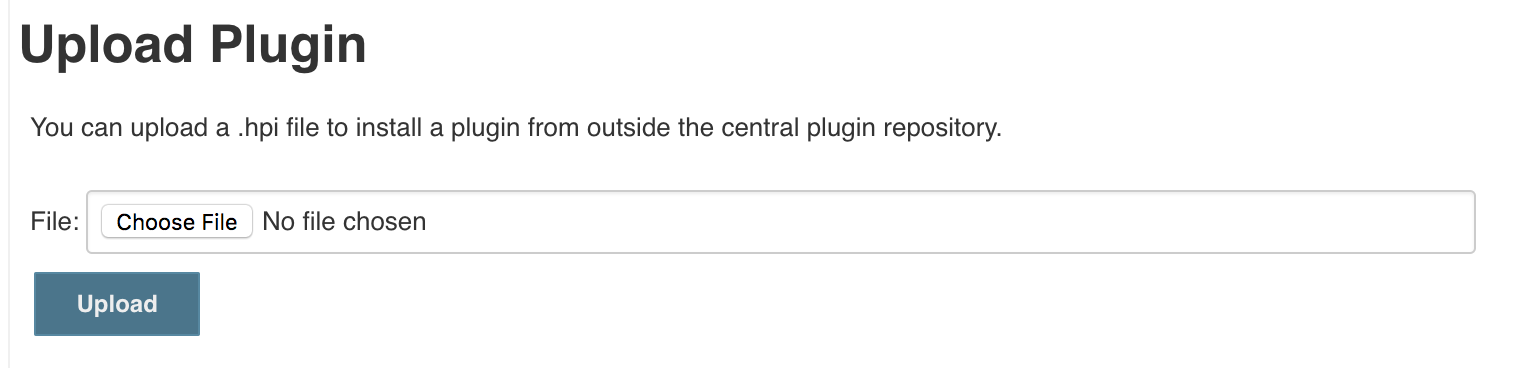
\includegraphics[width=0.9\textwidth]{grafiken/jenkins-plugin-03}
    \caption{Upload Plugin section}
    \label{fig:jenkins-plugin-03}
\end{figure}

There click on choose file and select the hpi file \textit{simile-jenkins-plugin.hpi} provided with the CD.
% \newpage
% \input{kapitel/methodologyQuestionMappingTable}
% 
% \input{kapitel/question_origins}
% \include{extern/fragebogenE}
% \include{extern/fragebogenD}
% 
% \input{kapitel/invitationLetters}
% 
% 
% \include{kapitel/coverageTable}

\selectlanguage{ngerman}
%Eidesstattliche Erklaerung
\chapter*{Eidesstattliche Erkl\"{a}rung}
\thispagestyle{empty}
Hiermit versichere ich, dass diese Abschlussarbeit von mir persönlich verfasst
ist und dass ich keinerlei fremde Hilfe in Anspruch genommen habe. Ebenso
versichere ich, dass diese Arbeit oder Teile daraus weder von mir selbst noch
von anderen als Leistungsnachweise andernorts eingereicht wurden. Wörtliche oder
sinn\-gemäße Übernahmen aus anderen Schriften und Veröffentlichungen in gedruckter
oder elektronischer Form sind gekennzeichnet. Sämtliche Sekundärliteratur und
sonstige Quellen sind nachgewiesen und in der Bibliographie aufgeführt. Das
Glei\-che gilt für graphische Darstellungen und Bilder sowie für alle
Internet-Quellen.

Ich bin ferner damit einverstanden, dass meine Arbeit zum Zwecke eines
Plagiatsabgleichs in elektronischer Form anonymisiert versendet und gespeichert
werden kann. Mir ist bekannt, dass von der Korrektur der Arbeit abgesehen werden
kann, wenn die Erklärung nicht erteilt wird.
\bigskip

\raggedright{Ort, den Datum} \bigskip \bigskip \bigskip

Martin Mustermann

\end{document}
